% !TeX program = xelatex
% ============================================================
%  《系统开发工具基础》实验报告 —— 第 2 周
%  姓名：徐宜安  学号：25060012033
%  编译：latexmk -pdf -halt-on-error 实验报告.tex
% ============================================================
\documentclass[12pt,a4paper,fontset=fandol]{ctexart}

% ---------- 页面布局 ----------
\usepackage[a4paper,margin=2.3cm]{geometry}
\setlength{\headheight}{14pt}
\setlength{\emergencystretch}{3em}

% ---------- 数学 ----------
\usepackage{amsmath,amssymb}

% ---------- 图片 ----------
\usepackage{graphicx}
\graphicspath{{课上/q05/}{课上/q06/}{课上/q07/}{课上/q08/}}
\usepackage{caption}
\captionsetup{font=small,labelfont=bf,labelsep=quad}
\usepackage{placeins}
\makeatletter
\setlength{\@fpsep}{12pt}
\makeatother

% ---------- 表格 ----------
\usepackage{booktabs,array,multirow}

% ---------- 颜色与代码高亮 ----------
\usepackage{xcolor}
\definecolor{codebg}{HTML}{f6f8fa}
\definecolor{codeframe}{HTML}{d0d7de}
\definecolor{kwred}{HTML}{cf222e}
\definecolor{strblue}{HTML}{0a3069}
\definecolor{cmtgray}{HTML}{6e7781}
\definecolor{fnpurple}{HTML}{8250df}
\definecolor{numblue}{HTML}{0550ae}

\usepackage{listings}
\renewcommand{\lstlistingname}{代码}

\lstdefinelanguage{shell}{
  morekeywords={mkdir,cd,echo,touch,cp,rm,mv,find,chmod,pwd,ls,cat,head,tail,sort,uniq,awk,sed,grep,printf,exit,return,if,then,else,elif,fi,do,done,for,in,while,case,esac,trap,sleep,bg,jobs,kill,wait,set,export,source,local,time},
  morekeywords=[2]{git,init,add,commit,checkout,merge,log,status,branch,clone,push,pull,diff,stash,restore,switch},
  morecomment=[l]{\#},
  morestring=[b]",
  morestring=[b]',
  sensitive=true,
}

\lstdefinelanguage{py}{
  morekeywords={import,from,def,return,if,else,elif,for,in,while,print,with,open,as,class,assert,random,seed,range,lambda,set},
  morecomment=[l]{\#},
  morestring=[b]",
  morestring=[b]',
  sensitive=true,
}

\lstdefinestyle{labcode}{
  backgroundcolor=\color{codebg},
  basicstyle=\small\ttfamily,
  keywordstyle=\color{kwred}\bfseries,
  keywordstyle=[2]\color{fnpurple}\bfseries,
  commentstyle=\color{cmtgray}\itshape,
  stringstyle=\color{strblue},
  numberstyle=\tiny\color{cmtgray},
  numbers=left,
  frame=single,
  rulecolor=\color{codeframe},
  breaklines=true,
  breakatwhitespace=false,
  showstringspaces=false,
  tabsize=4,
  columns=fullflexible,
  keepspaces=true,
  captionpos=b,
  xleftmargin=1.6em,
  framexleftmargin=1.2em,
  aboveskip=0.6em,
  belowskip=0.6em,
}
\lstset{style=labcode}

% ---------- 页眉页脚 ----------
\usepackage{fancyhdr}
\usepackage{lastpage}
\pagestyle{fancy}
\fancyhf{}
\fancyhead[L]{\small 系统开发工具基础 · 实验报告}
\fancyhead[R]{\small 徐宜安\quad 25060012033}
\fancyfoot[C]{\small 第 \thepage\ 页 / 共 \pageref{LastPage} 页}
\renewcommand{\headrulewidth}{0.4pt}

% ---------- 超链接 ----------
\usepackage{hyperref}
\hypersetup{colorlinks=true,linkcolor=numblue,urlcolor=numblue,citecolor=numblue}

% ---------- 题目要求框 ----------
\usepackage{tcolorbox}
\tcbuselibrary{breakable}
\newtcolorbox{taskbox}[1][]{
  colback=blue!4!white,
  colframe=blue!50!black,
  fonttitle=\bfseries,
  title={#1},
  boxrule=0.6pt,
  arc=1.5pt,
  left=8pt,right=8pt,top=5pt,bottom=5pt,
  breakable,
}

% ---------- 列表 ----------
\usepackage{enumitem}

% ==================== 每周填写区 ====================
\newcommand{\weeknum}{第 2 周}
\newcommand{\weektheme}{命令行环境 · 开发环境与工具 · Debugging and Profiling}
\newcommand{\classdate}{2026 年 8 月 31 日}
% ==================== 每周填写区结束 ====================

\newcommand{\makereporttitle}{%
  \begin{center}
    {\LARGE\bfseries 系统开发工具基础 · 实验报告}\\[0.4em]
    {\normalsize \weeknum：\weektheme}\\[0.7em]
    {\small
    \begin{tabular}{@{}ll@{\hspace{3em}}ll@{}}
      姓\quad 名 & 徐宜安 & 学\quad 号 & 25060012033 \\
      授课教师 & 周小伟 & 上课日期 & \classdate \\
      Git 仓库 & \href{https://github.com/xya-123/Fundamentals-of-Computer-System-Development-Tools}{GitHub 课程仓库} & 报告日期 & \today \\
    \end{tabular}}\\[0.7em]
    \rule{\textwidth}{0.8pt}
  \end{center}
}

\begin{document}
\makereporttitle

\section{课上练习}

% ================= q05 =================
\subsection{q05 · 控制一个可清理的后台任务（进程、信号与任务控制）}

\begin{taskbox}[题目要求]
将给定脚本保存为 \texttt{worker.sh}，并完成以下操作：
\begin{itemize}[nosep]
  \item 赋予脚本执行权限，在前台启动，将 stdout、stderr 分别写入两个日志文件；
  \item 使用 Ctrl-Z 挂起任务，再通过 \texttt{bg} 放到后台，使用 \texttt{jobs} 确认状态；
  \item 用 \texttt{jobs -p} 取得 PID，发送 SIGTERM 并等待任务结束；
  \item 确认 \texttt{cleanup.log} 中出现 \texttt{CLEAN\_EXIT}，且任务已经退出。
\end{itemize}
\end{taskbox}

\lstinputlisting[language=shell,caption={worker.sh：带信号清理逻辑的后台任务},label={lst:q05-worker}]{课上/q05/worker.sh}

\textbf{实验过程：} 先用 \texttt{chmod +x worker.sh} 增加执行权限，随后运行
\texttt{./worker.sh}，并分别用 \texttt{1>stdout.log} 和 \texttt{2>stderr.log}
重定向标准输出、标准错误。
运行后按 Ctrl-Z 后任务进入
\texttt{Stopped} 状态，再执行 \texttt{bg}，\texttt{jobs} 显示它已在后台继续运行。
最后使用 \texttt{kill \$(jobs -p)} 直接取得后台任务 PID 并发送 SIGTERM。
完整操作见图~\ref{fig:q05-process}。

\begin{figure}[htbp]
  \centering
  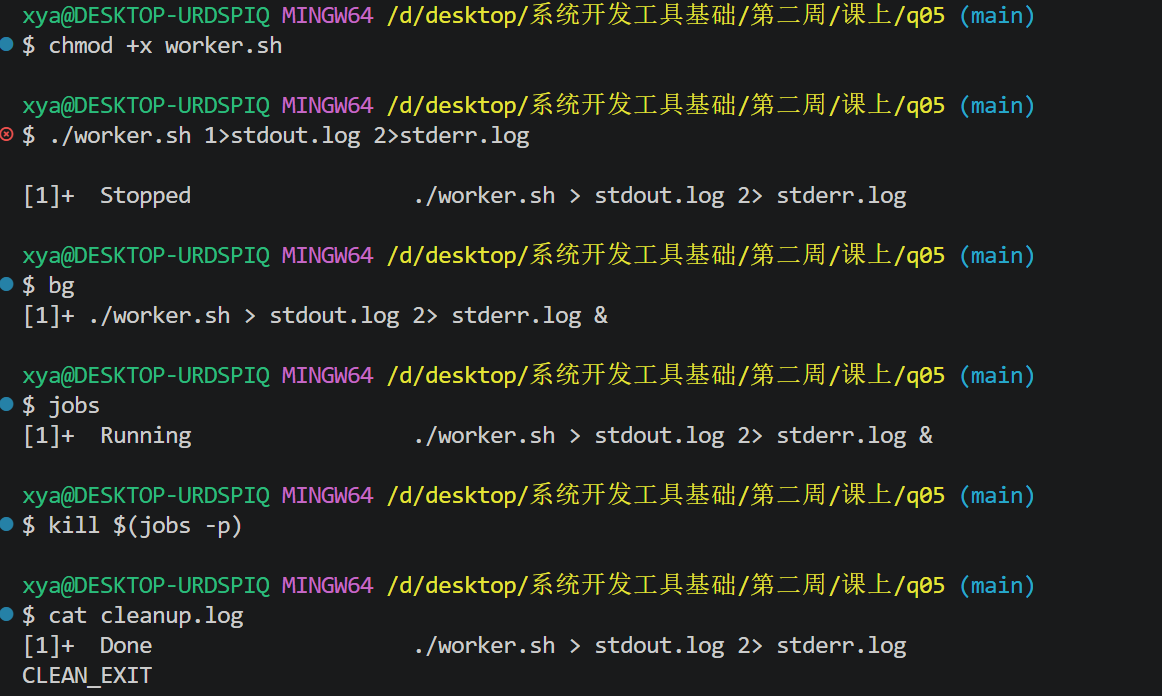
\includegraphics[width=0.94\textwidth]{课上/q05/截图.png}
  \caption{q05 任务挂起、后台恢复、发送信号与清理结果}
  \label{fig:q05-process}
\end{figure}

\textbf{实验结果：} 收到 SIGTERM 后，脚本执行 \texttt{trap} 中的清理命令并正常退出，
终端显示任务状态为 \texttt{Done}，\texttt{cleanup.log} 中写入了
\texttt{CLEAN\_EXIT}。\texttt{stdout.log} 保存了 0 到 12（与任务的运行时间有关），
\texttt{stderr.log} 为空，说明标准输出和标准错误已正确分开。

\FloatBarrier

% ================= q06 =================
\subsection{q06 · 语义重构与本地开发反馈（开发环境与工具）}

\begin{taskbox}[题目要求]
在 q06 中创建给定的三个 Python 文件，并完成以下操作：
\begin{itemize}[nosep]
  \item 配置 Python、pytest、ruff 和 Python 语言服务器；
  \item 演示跳转到定义和查找引用；
  \item 使用“重命名符号”把 \texttt{total\_price} 改为 \texttt{calculate\_total}，同步修改定义和全部引用；
  \item 临时加入未使用的 \texttt{import os}，用 ruff 找出并删除，最后保证 ruff 和 pytest 均通过。
\end{itemize}
\end{taskbox}

\textbf{实验过程：} 首先确认 Python、pytest、ruff 的版本，并检查 VS Code 中的
Python、Pylance 和 Python Debugger 插件，环境配置见图~\ref{fig:q06-env}。

\begin{figure}[htbp]
  \centering
  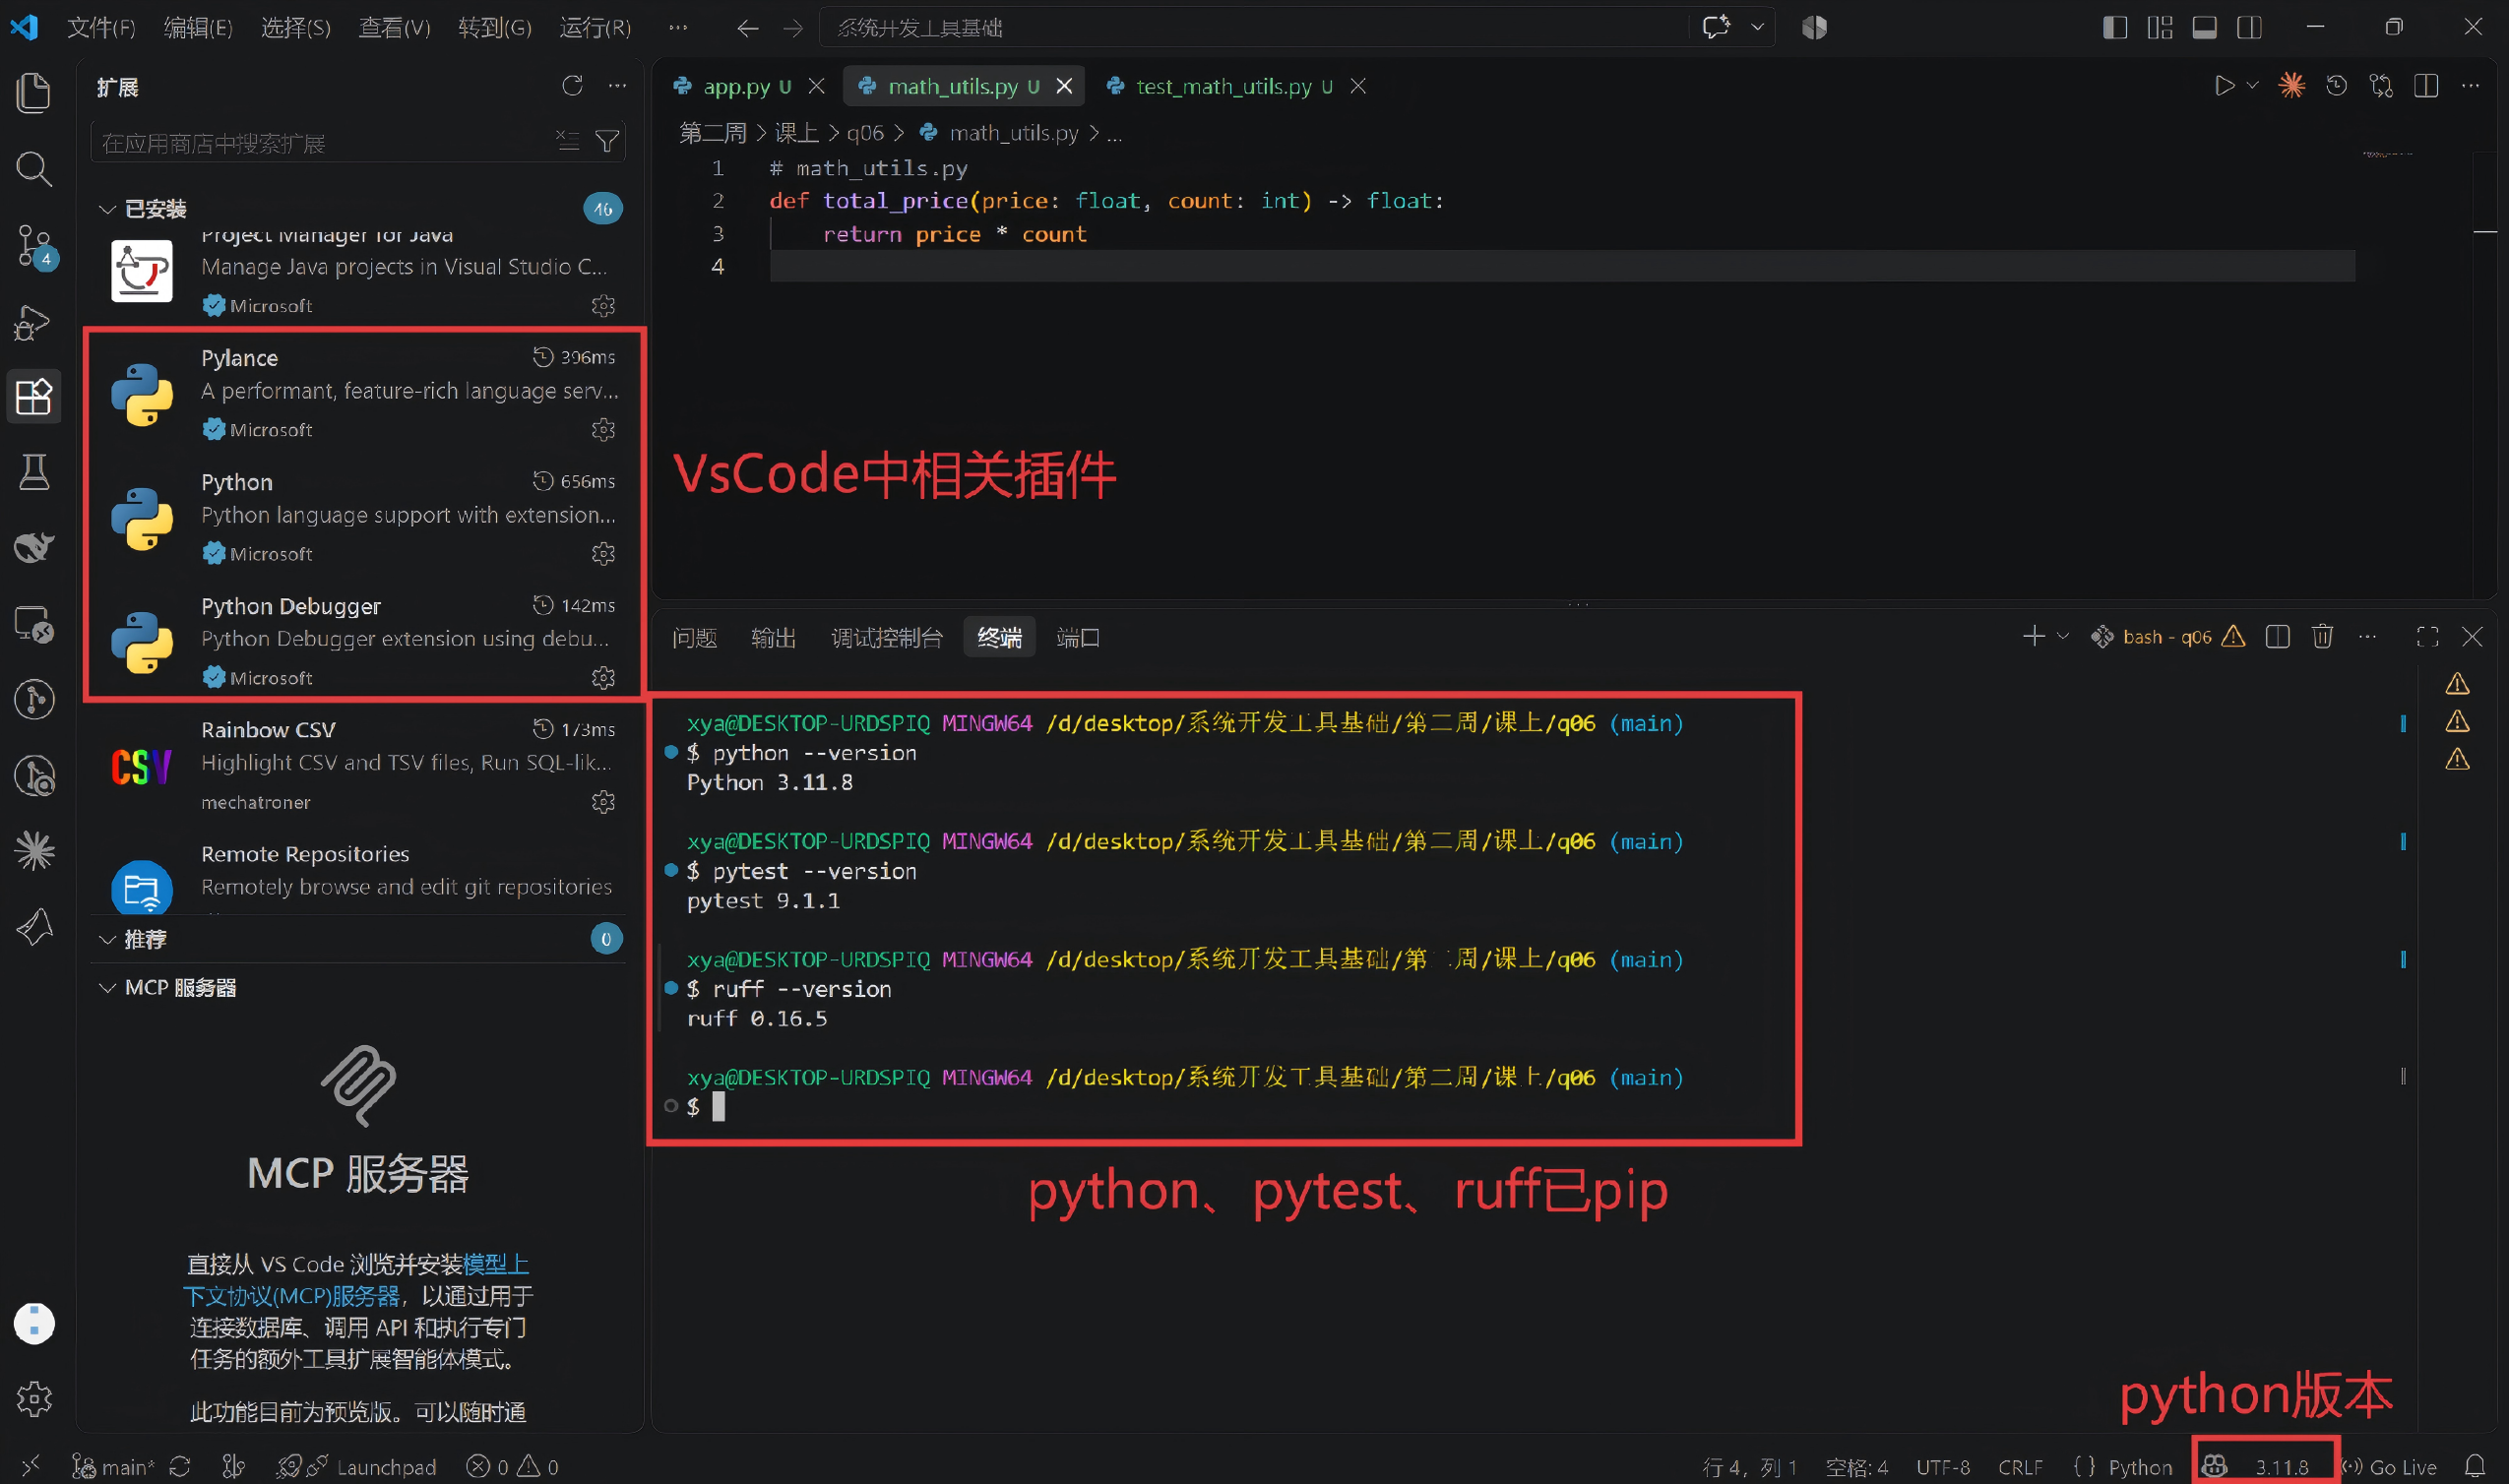
\includegraphics[width=0.94\textwidth]{课上/q06/图1-配置好Python、pytest、ruff以及下载好VsCode相关插件.png}
  \caption{q06 Python 工具版本与 VS Code 插件配置}
  \label{fig:q06-env}
\end{figure}

在 \texttt{app.py} 中按住 Ctrl 点击 \texttt{total\_price}，编辑器能够定位到
\texttt{math\_utils.py} 中的函数定义（图~\ref{fig:q06-jump}）。随后鼠标右键点击 \texttt{total\_price}并在菜单中选择
“查找所有引用”，VS Code 在三个文件中找到 5 处结果，包括函数定义、两处导入和两处调用，
过程见图~\ref{fig:q06-refs}。

\begin{figure}[htbp]
  \centering
  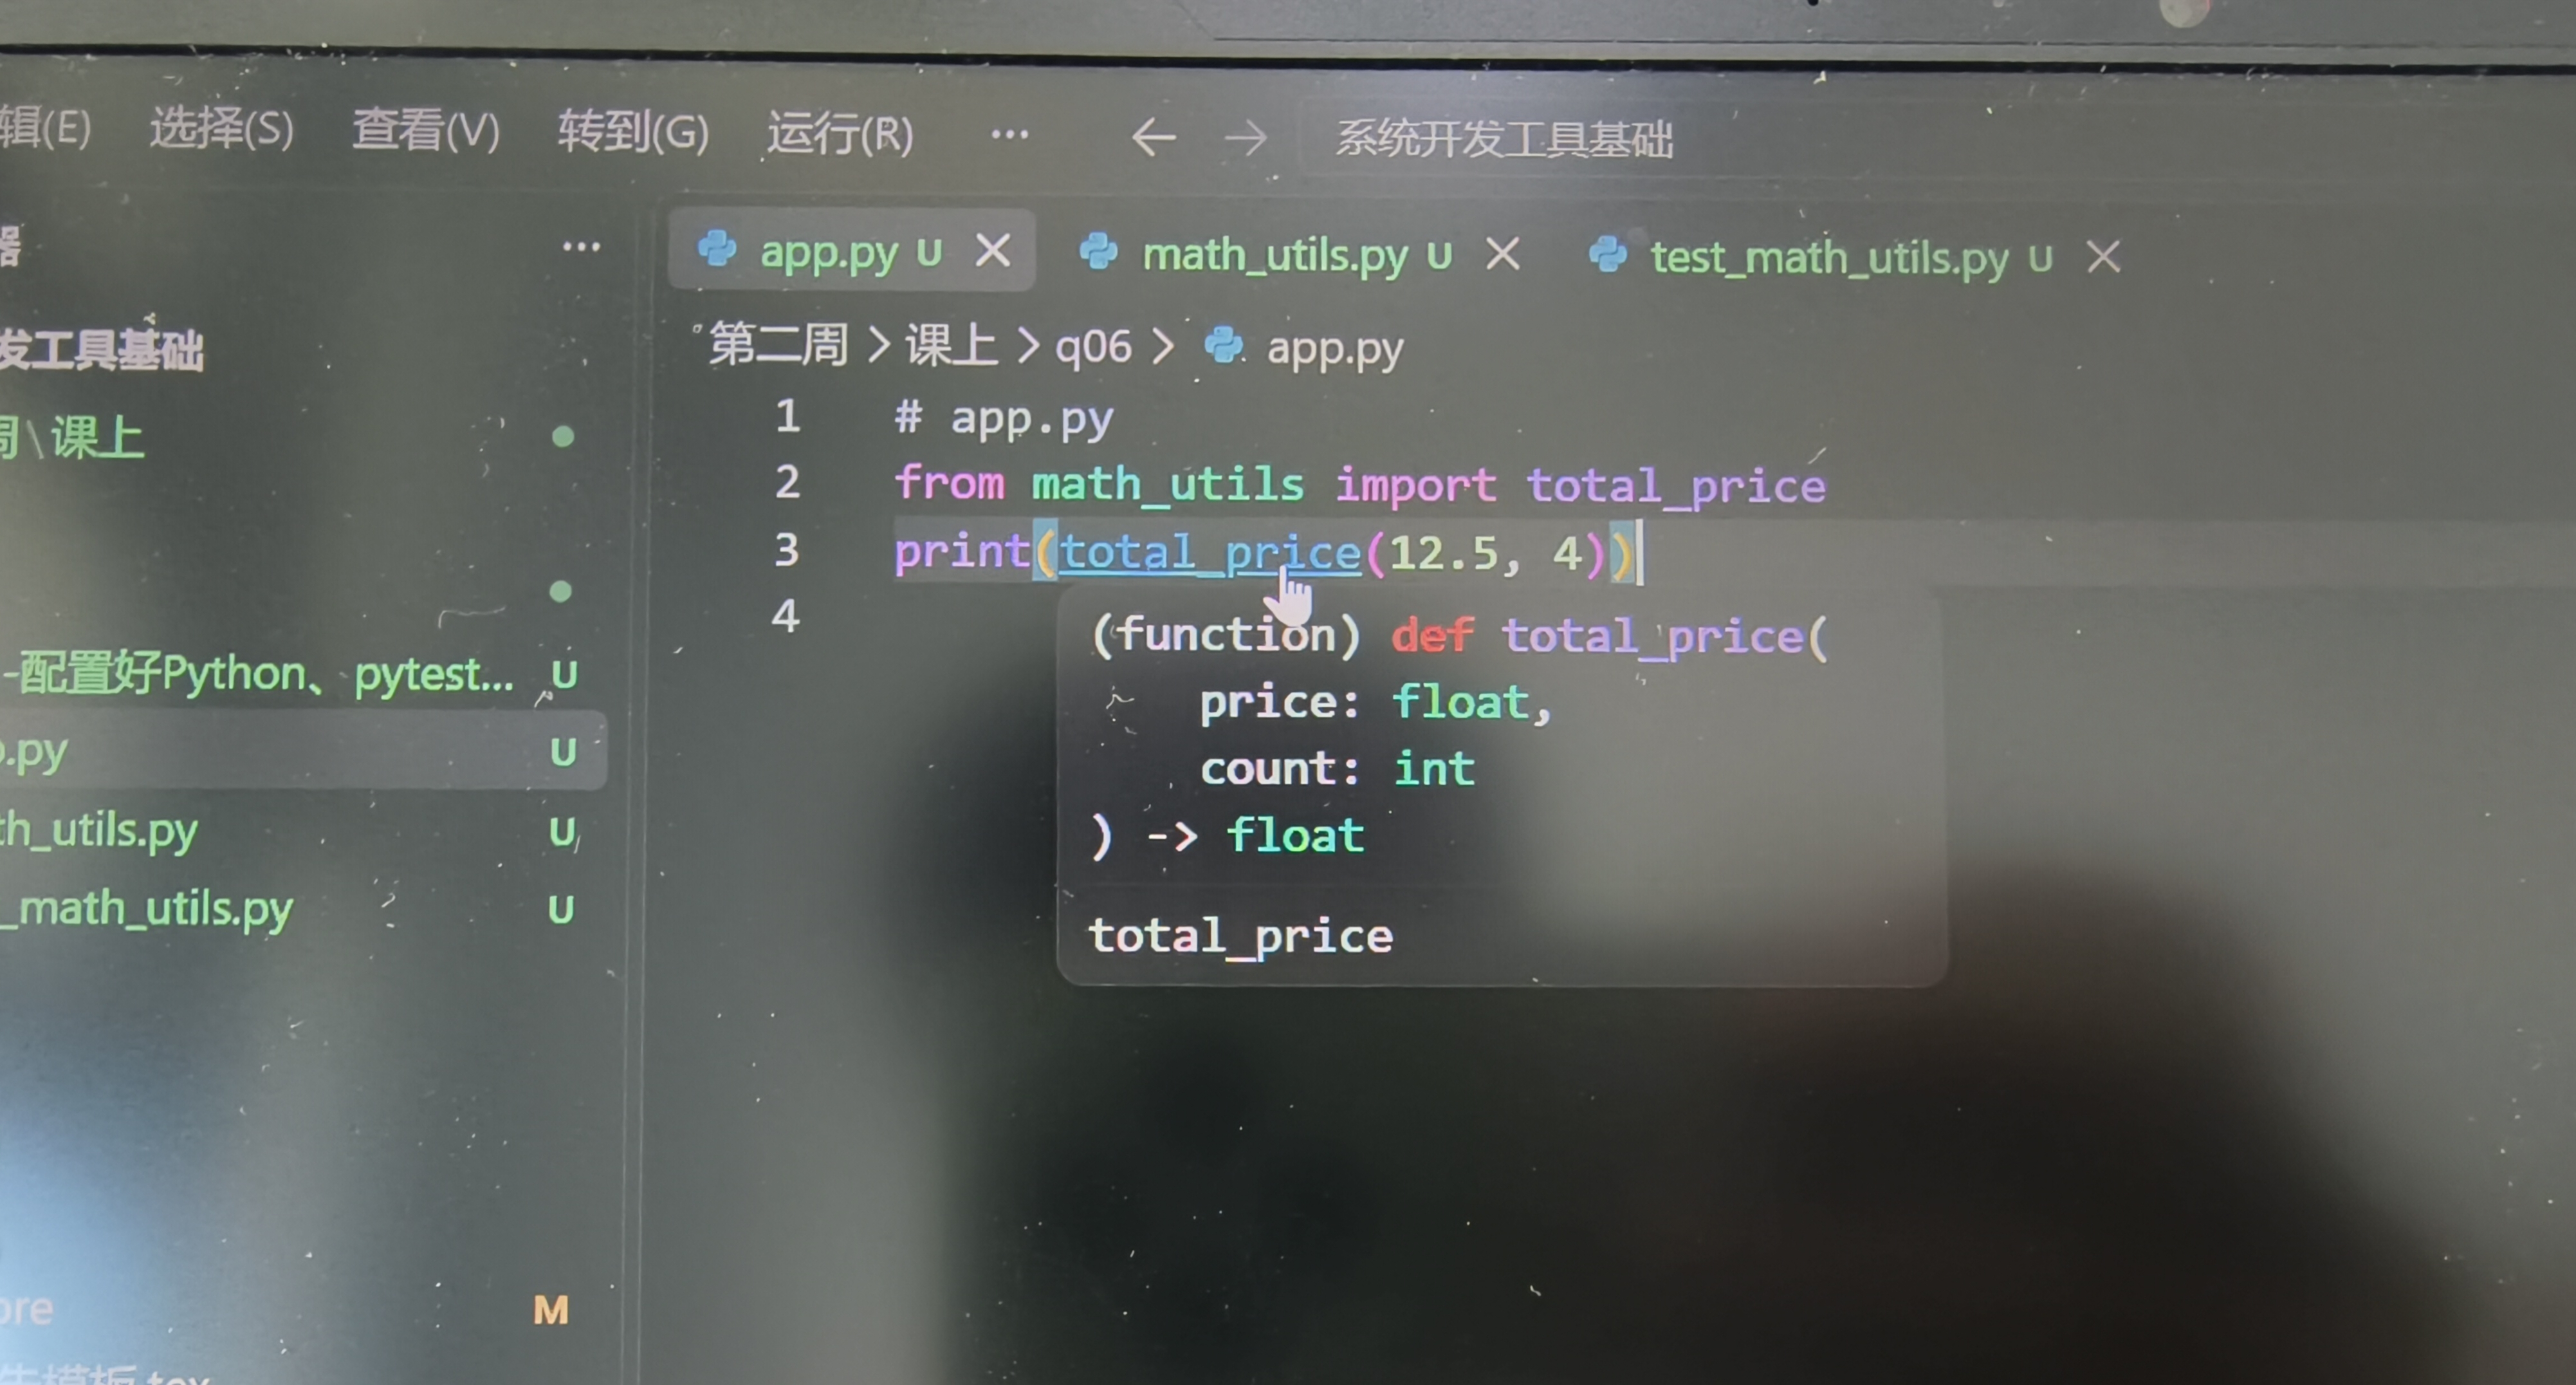
\includegraphics[width=0.70\textwidth]{课上/q06/图2-按住Ctrl可以点击跳转.jpg}
  \caption{按住 Ctrl 点击函数调用并跳转到定义}
  \label{fig:q06-jump}
\end{figure}

\begin{figure}[htbp]
  \centering
  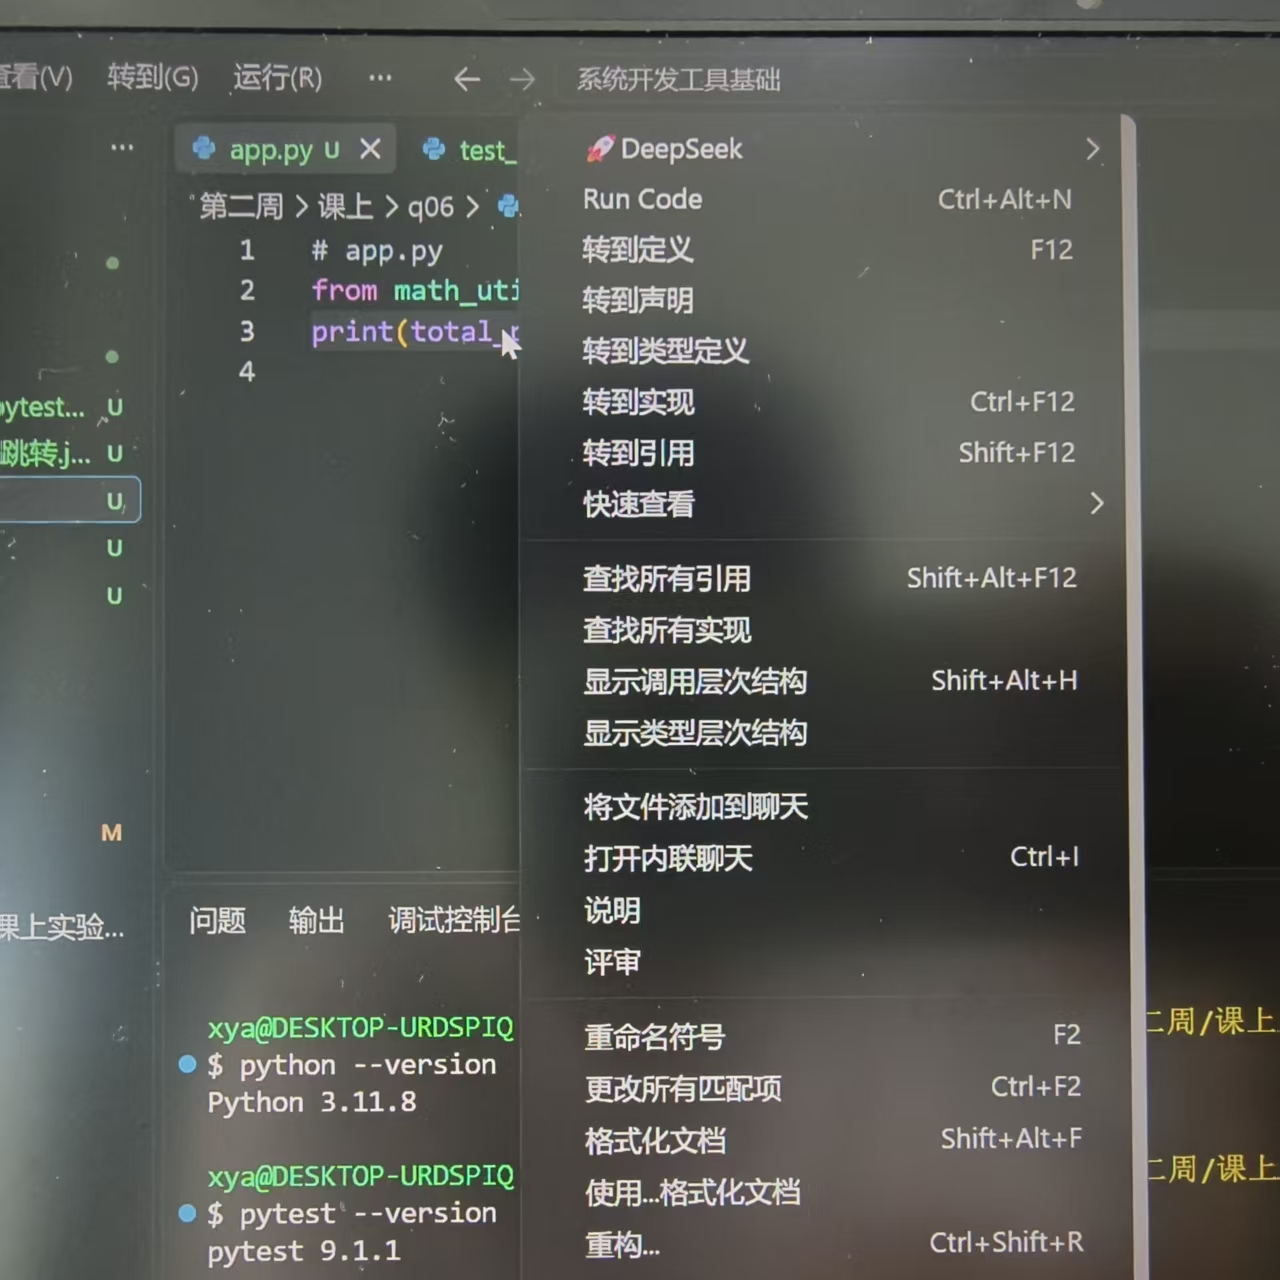
\includegraphics[trim=250bp 0 70bp 0,clip,height=0.23\textheight]{课上/q06/图3-1-鼠标放在 `total_price`上右键查找引用.jpg}\hfill
  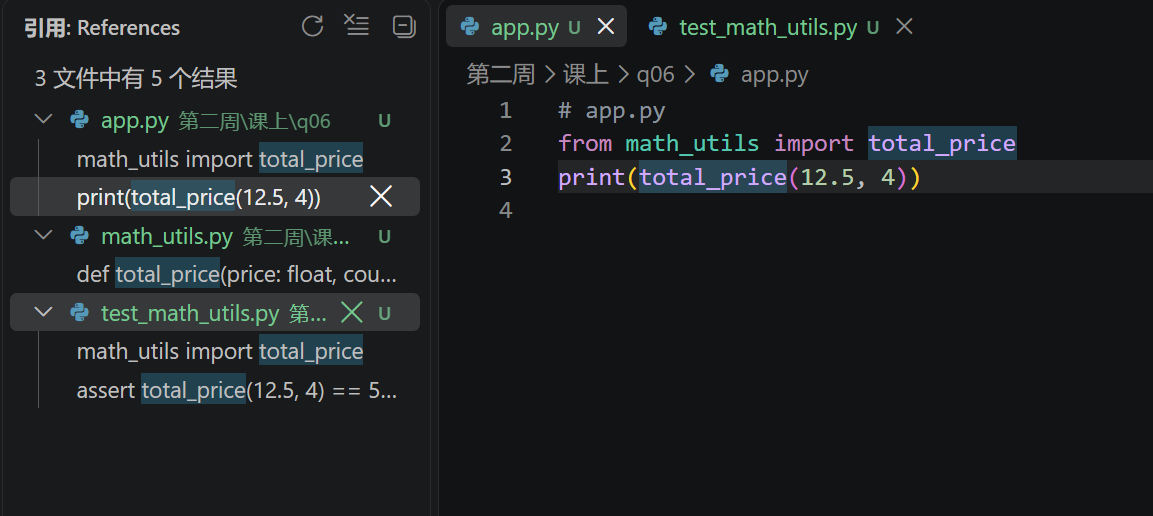
\includegraphics[height=0.21\textheight]{课上/q06/图3-2-查看所有的引用.png}
  \caption{从右键菜单查找引用，并列出三个文件中的 5 处结果}
  \label{fig:q06-refs}
\end{figure}

接着对函数右键选择“重命名符号”，输入新名称 \texttt{calculate\_total}。
这一步由语言服务器统一更新符号，没有替换 \texttt{test\_total\_price}，操作见图~\ref{fig:q06-rename}。

\begin{figure}[htbp]
  \centering
  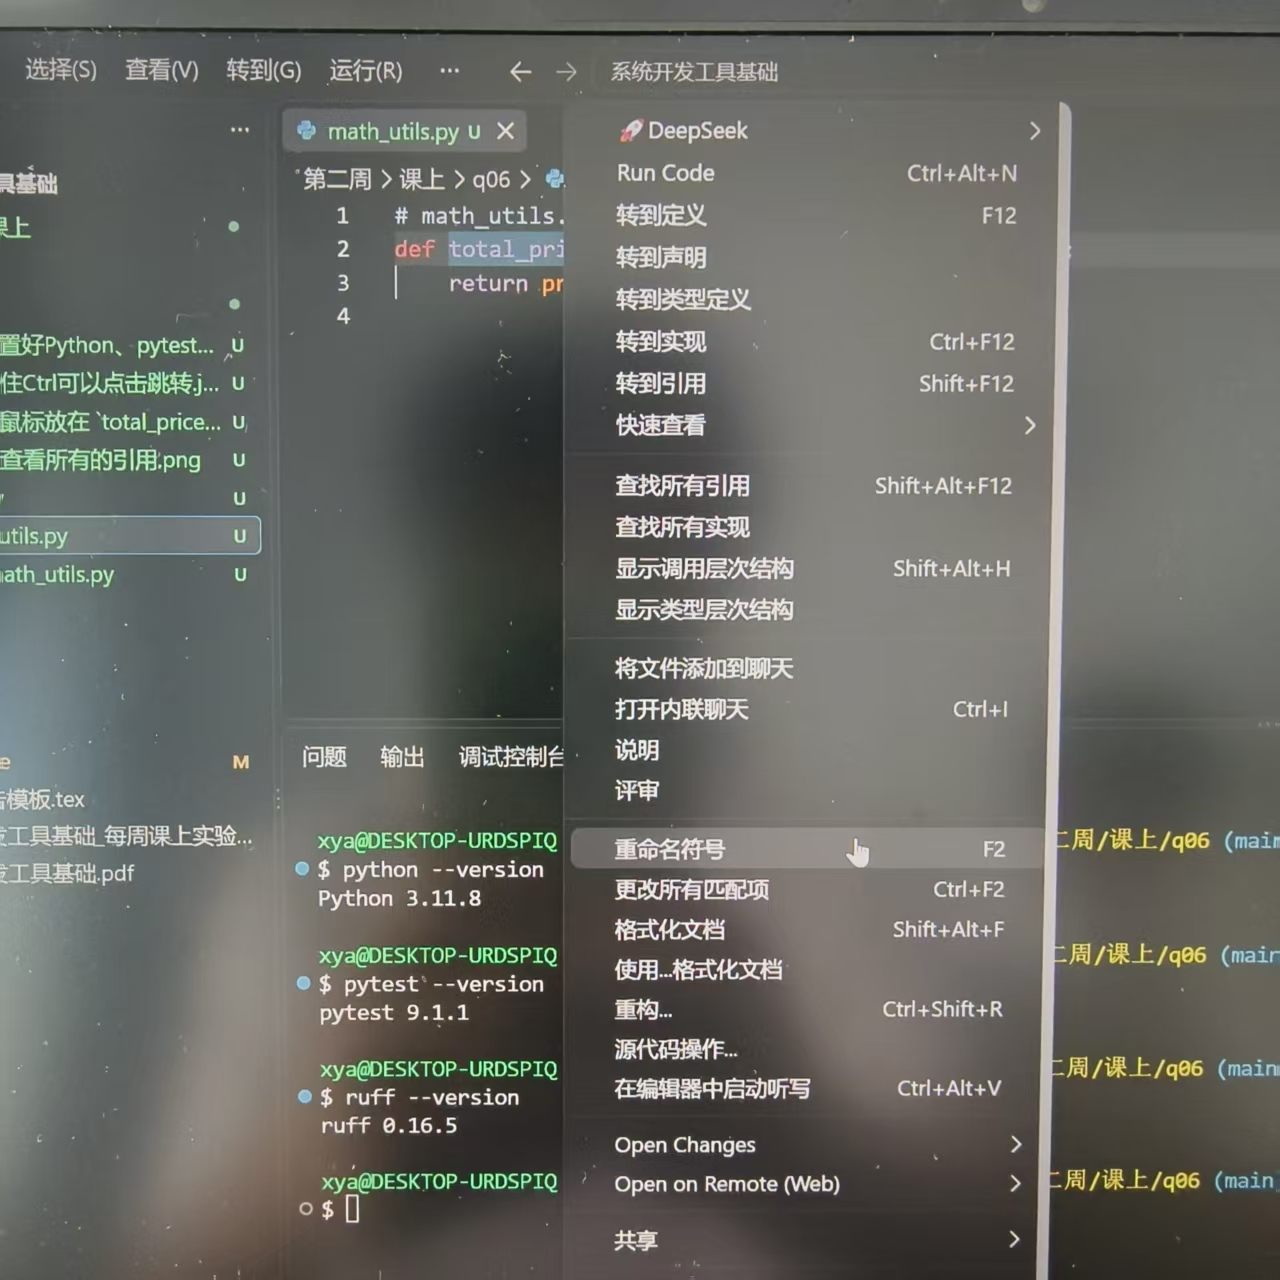
\includegraphics[trim=260bp 0 90bp 0,clip,height=0.28\textheight]{课上/q06/图4-1-重命名符号（右键选择这一项或者快捷键F2）.jpg}\hfill
  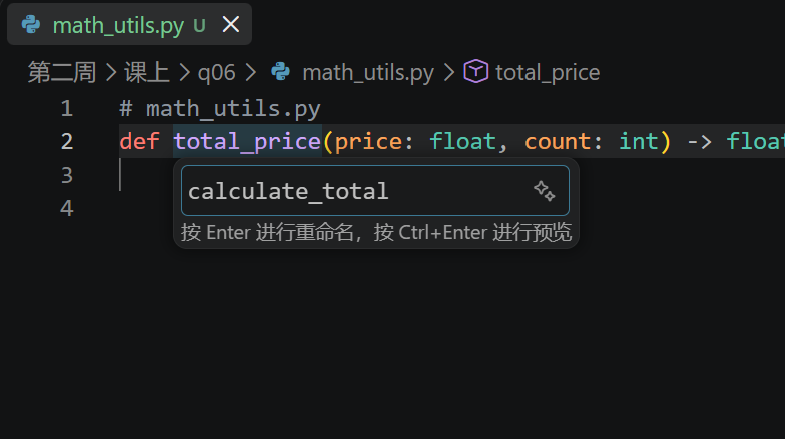
\includegraphics[height=0.23\textheight]{课上/q06/图4-2-重命名.png}
  \caption{使用“重命名符号”将函数名改为 calculate\_total}
  \label{fig:q06-rename}
\end{figure}

重命名后的三个文件如下。

\lstinputlisting[language=py,basicstyle=\footnotesize\ttfamily,caption={math\_utils.py：重命名后的函数定义},label={lst:q06-math}]{课上/q06/math_utils.py}
\lstinputlisting[language=py,basicstyle=\footnotesize\ttfamily,caption={app.py：重命名后的导入与调用},label={lst:q06-app}]{课上/q06/app.py}
\lstinputlisting[language=py,basicstyle=\footnotesize\ttfamily,caption={test\_math\_utils.py：同步更新后的测试},label={lst:q06-test}]{课上/q06/test_math_utils.py}

最后在 \texttt{app.py} 中临时加入 \texttt{import os}。第一次执行
\texttt{ruff check .} 时，ruff 报告导入顺序问题和未使用的 \texttt{os}，并指出
\texttt{F401} 的具体位置（图~\ref{fig:q06-ruff-error}）。用
\texttt{ruff check . --fix} 修复相关问题，再重新运行检查和测试。

\begin{figure}[htbp]
  \centering
  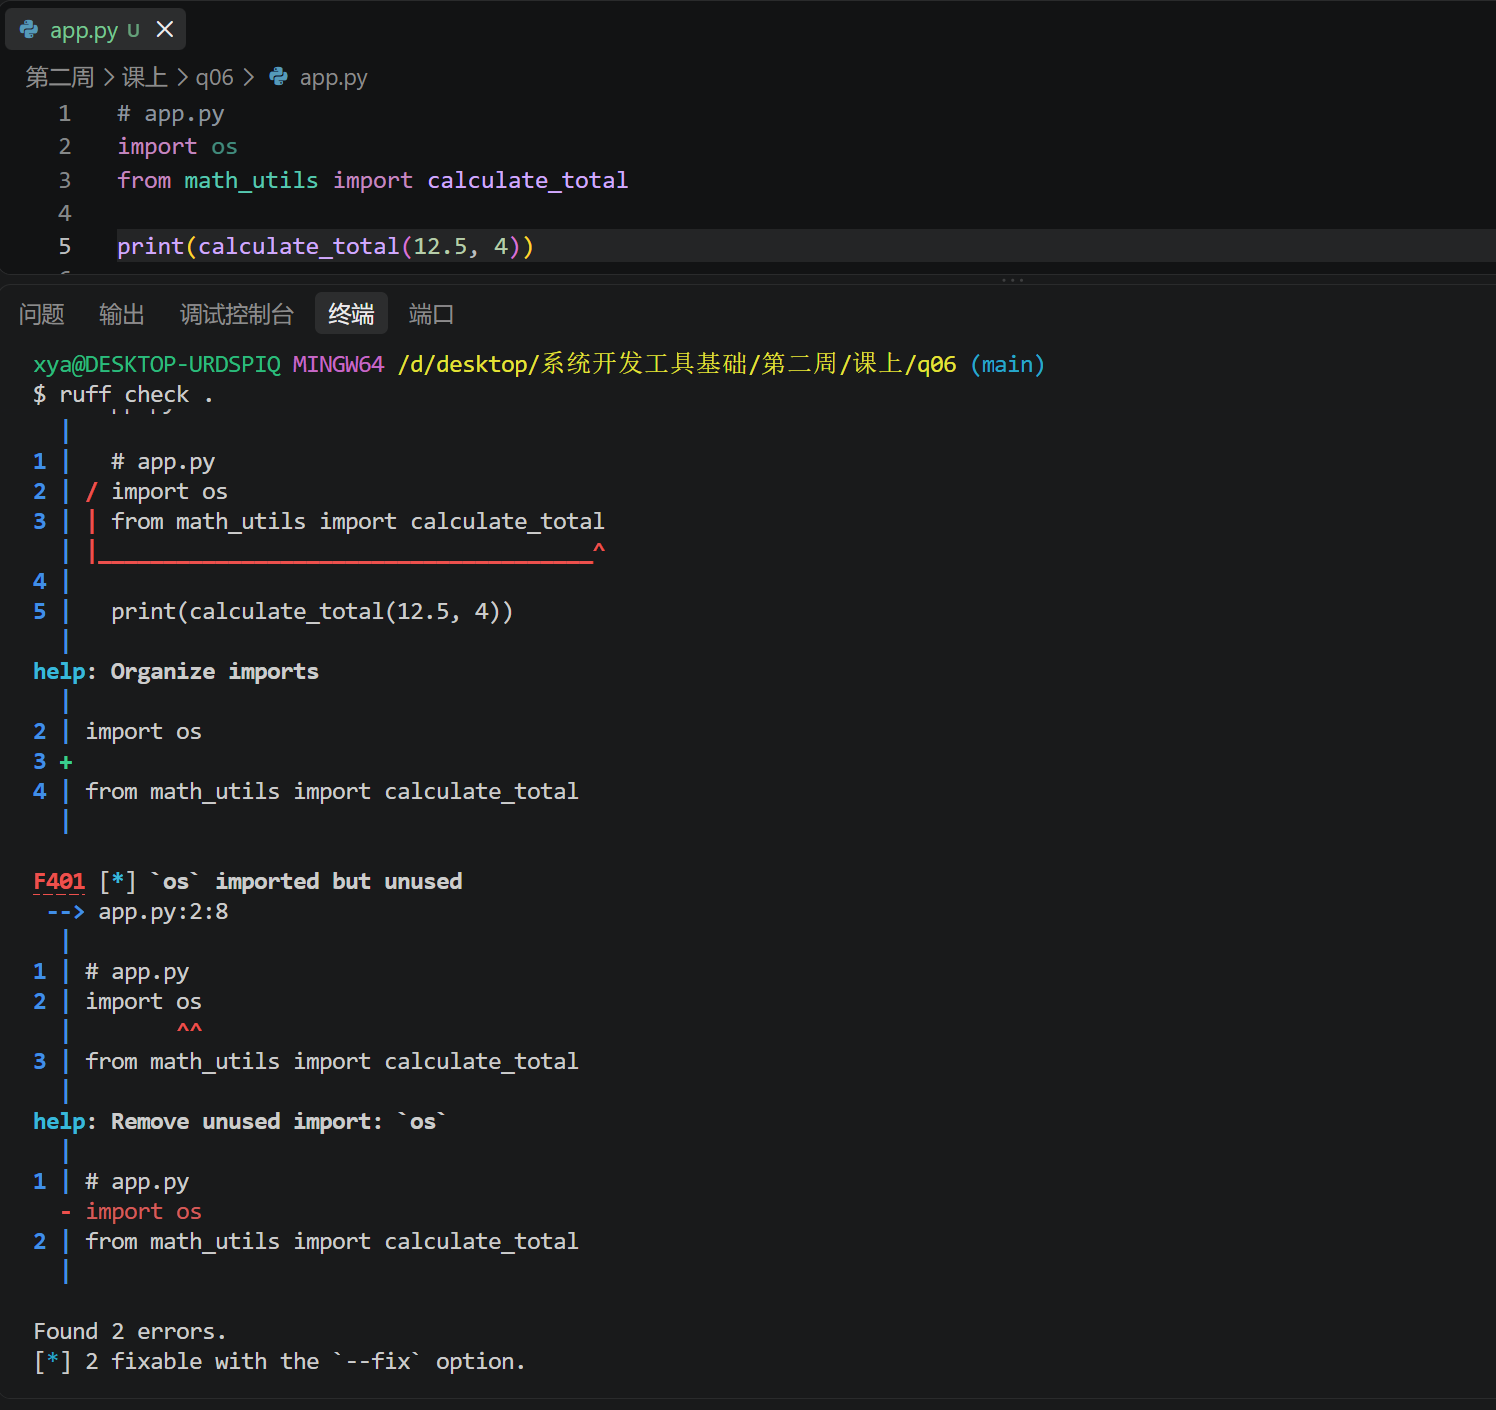
\includegraphics[height=0.53\textheight]{课上/q06/图5-1-ruff找出错误.png}
  \caption{ruff 检出未使用的 os 和导入顺序问题}
  \label{fig:q06-ruff-error}
\end{figure}

\begin{figure}[htbp]
  \centering
  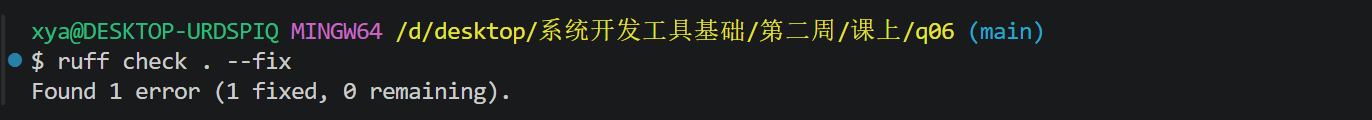
\includegraphics[width=0.95\textwidth]{课上/q06/图5-2-ruff修复，确认都无问题.png}\\[-0.2em]
  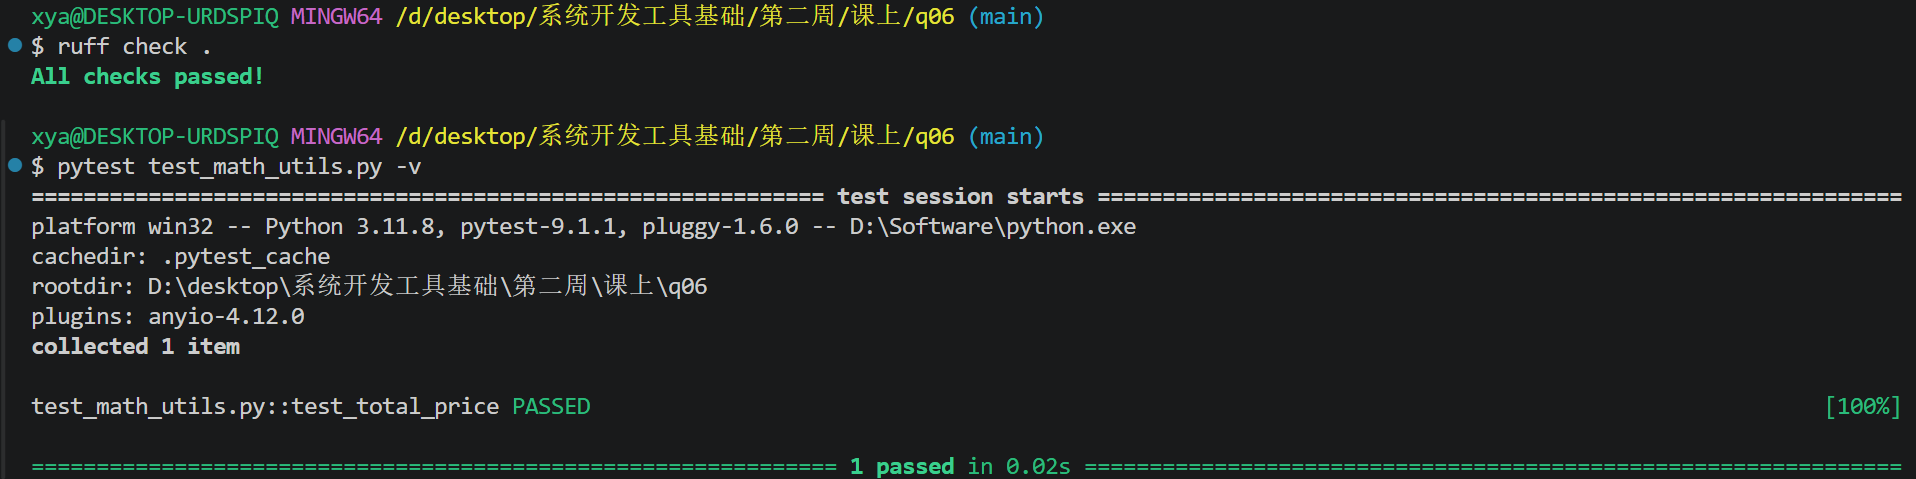
\includegraphics[width=0.95\textwidth]{课上/q06/图6-最终跑ruff和pytest.png}
  \caption{ruff 自动修复后再次检查，并运行 pytest 验证}
  \label{fig:q06-final}
\end{figure}

\textbf{实验结果：} 最终 \texttt{ruff check .} 输出 \texttt{All checks passed!}，
pytest 收集并通过 1 个测试，耗时 0.02 s（图~\ref{fig:q06-final}）。
函数改名后仍能正确计算 \(12.5\times4=50.0\)，说明语义重构没有破坏原有功能。

\FloatBarrier

% ================= q07 =================
\subsection{q07 · 用调试器定位归并排序缺陷（Debugging）}

\begin{taskbox}[题目要求]
运行给定的归并排序代码，使用调试器定位并修复缺陷：
\begin{itemize}[nosep]
  \item 先运行给定输入，确认结果错误或出现异常；
  \item 在 \texttt{merge} 中设置断点，观察 \texttt{i}、\texttt{j}、\texttt{left[i]} 和 \texttt{right[j]}；
  \item 完成最小修复，不得使用 \texttt{sorted} 替换归并排序；
  \item 增加给定输入和含重复元素列表两个 pytest 测试，并保证测试通过。
\end{itemize}
\end{taskbox}

\textbf{实验过程：} 原程序运行后得到
\texttt{[1, 5, 4, 3, 4, 5, 6, 9]}，结果没有按升序排列，修复前的代码和输出见
图~\ref{fig:q07-before-after}(a)。

在 \texttt{merge} 的比较语句处设置断点，将 \texttt{left[i]} 和 \texttt{right[j]}
加入监视窗口。调试开始时 \texttt{i=j=0}。此时 \texttt{left=[3]}、\texttt{right=[1]}，
监视值分别为 3 和 1（图~\ref{fig:q07-debug}）。继续执行到
\texttt{left=[1,3]}、\texttt{right=[1,4]}、\texttt{i=j=1} 时，程序进入 else 分支，
却读取了 \texttt{right[i]}。此时左右列表下标刚好相同，所以没有立即报错，但代码使用的
下标与递增的 \texttt{j} 不一致，问题位置见图~\ref{fig:q07-bug}。

\begin{figure}[htbp]
  \centering
  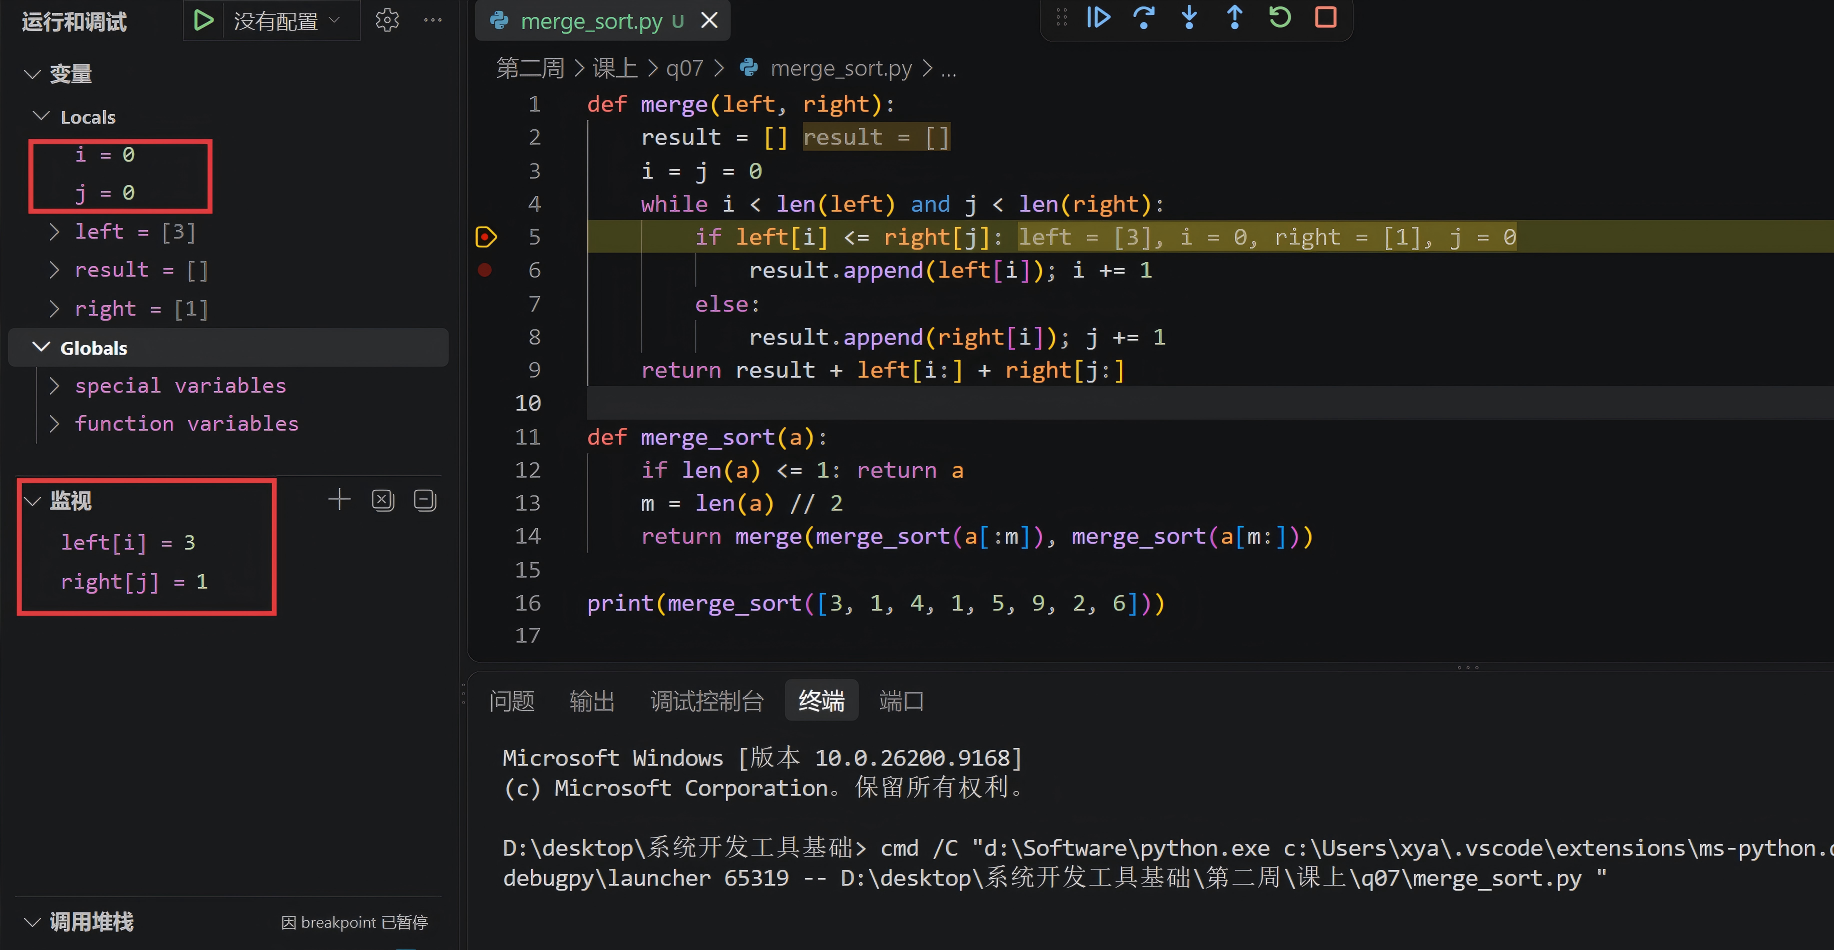
\includegraphics[width=0.96\textwidth]{课上/q07/图2-打断点调试，监视相关变量.png}
  \caption{在 merge 中设置断点并监视左右列表及其下标}
  \label{fig:q07-debug}
\end{figure}

\begin{figure}[htbp]
  \centering
  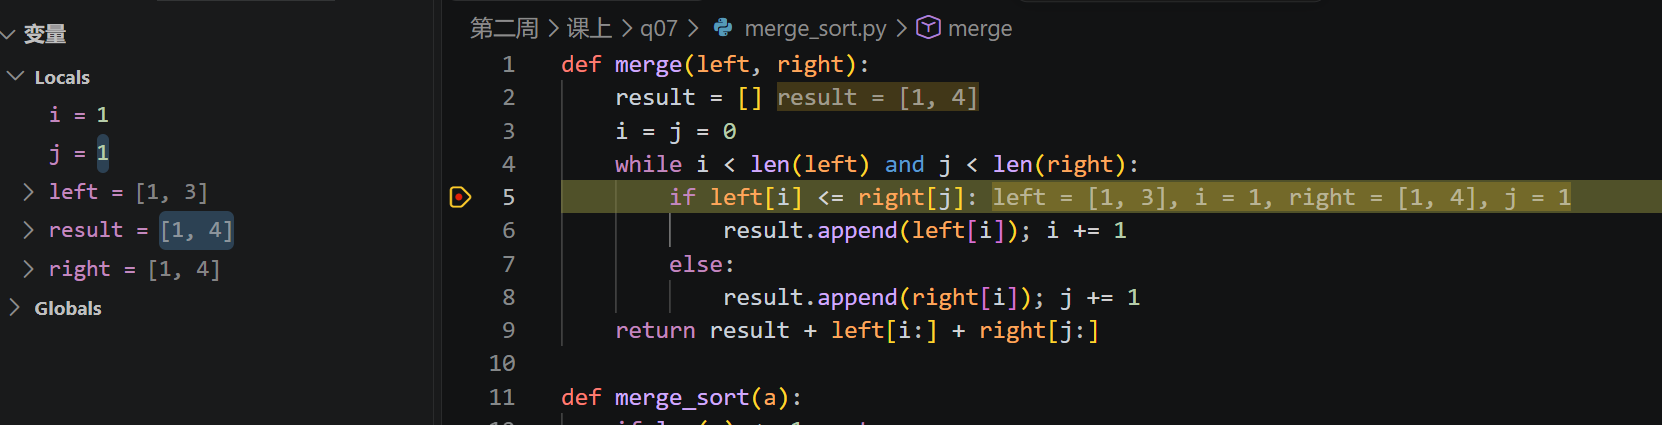
\includegraphics[width=0.94\textwidth]{课上/q07/图3-发现问题.png}
  \caption{调试过程中定位到 else 分支使用了错误下标 i}
  \label{fig:q07-bug}
\end{figure}

最小修复是把第 8 行的 \texttt{right[i]} 改成 \texttt{right[j]}，其余归并排序逻辑保持不变。
最终代码见代码~\ref{lst:q07-merge}。修复后再次运行同一输入，输出变为
\texttt{[1,1,2,3,4,5,6,9]}，见图~\ref{fig:q07-before-after}(b)。

\lstinputlisting[language=py,caption={merge\_sort.py：修复下标后的归并排序},label={lst:q07-merge}]{课上/q07/merge_sort.py}

\begin{figure}[htbp]
  \centering
  \begin{minipage}[t]{0.49\textwidth}
    \centering
    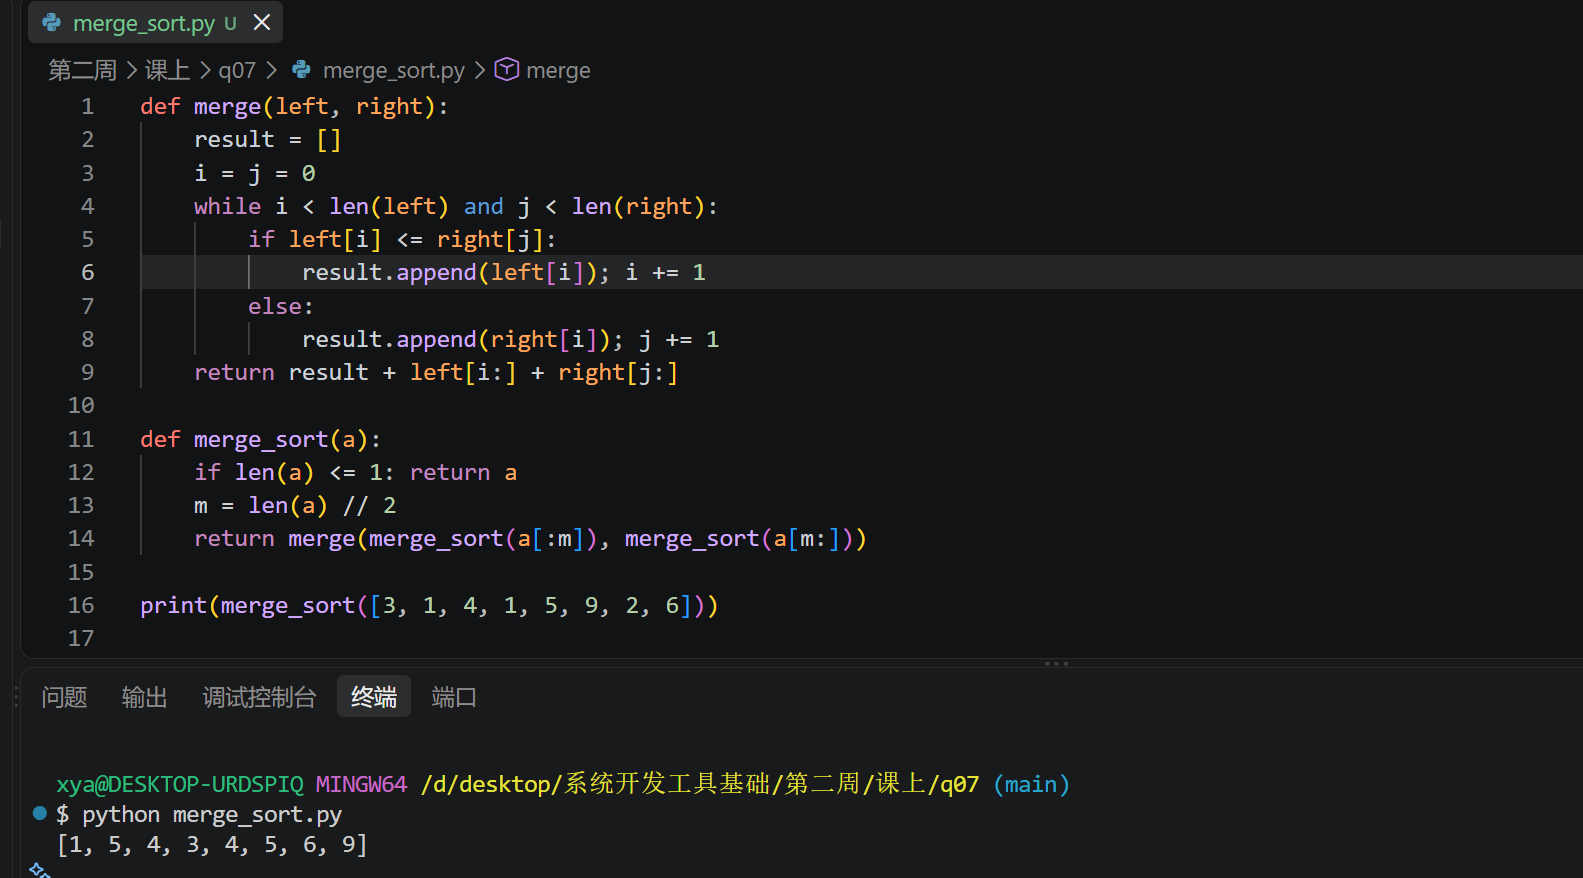
\includegraphics[width=\textwidth]{课上/q07/图1-确认原始结果异常.png}\\[-0.1em]
    \small (a) 修复前：输出没有正确排序
  \end{minipage}\hfill
  \begin{minipage}[t]{0.49\textwidth}
    \centering
    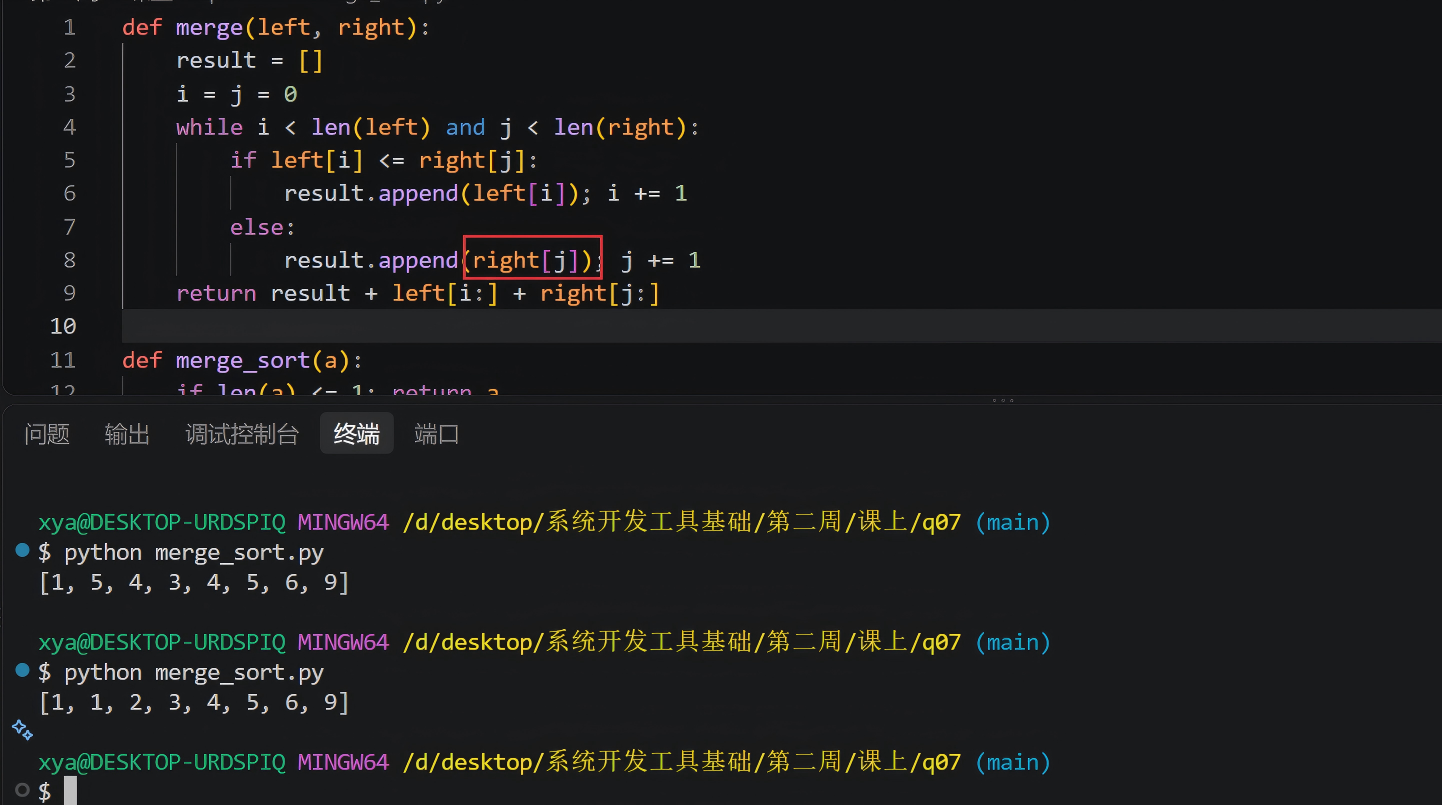
\includegraphics[width=\textwidth]{课上/q07/图4-修改代码结果正确.png}\\[-0.1em]
    \small (b) 修复后：同一输入得到升序结果
  \end{minipage}
  \caption{q07 修复前后的代码运行结果对比}
  \label{fig:q07-before-after}
\end{figure}

随后在 \texttt{test\_merge.py} 中加入两个测试，分别覆盖题目给定输入和包含多个重复元素的列表。

\lstinputlisting[language=py,caption={test\_merge.py：给定输入与重复元素测试},label={lst:q07-test}]{课上/q07/test_merge.py}

\begin{figure}[htbp]
  \centering
  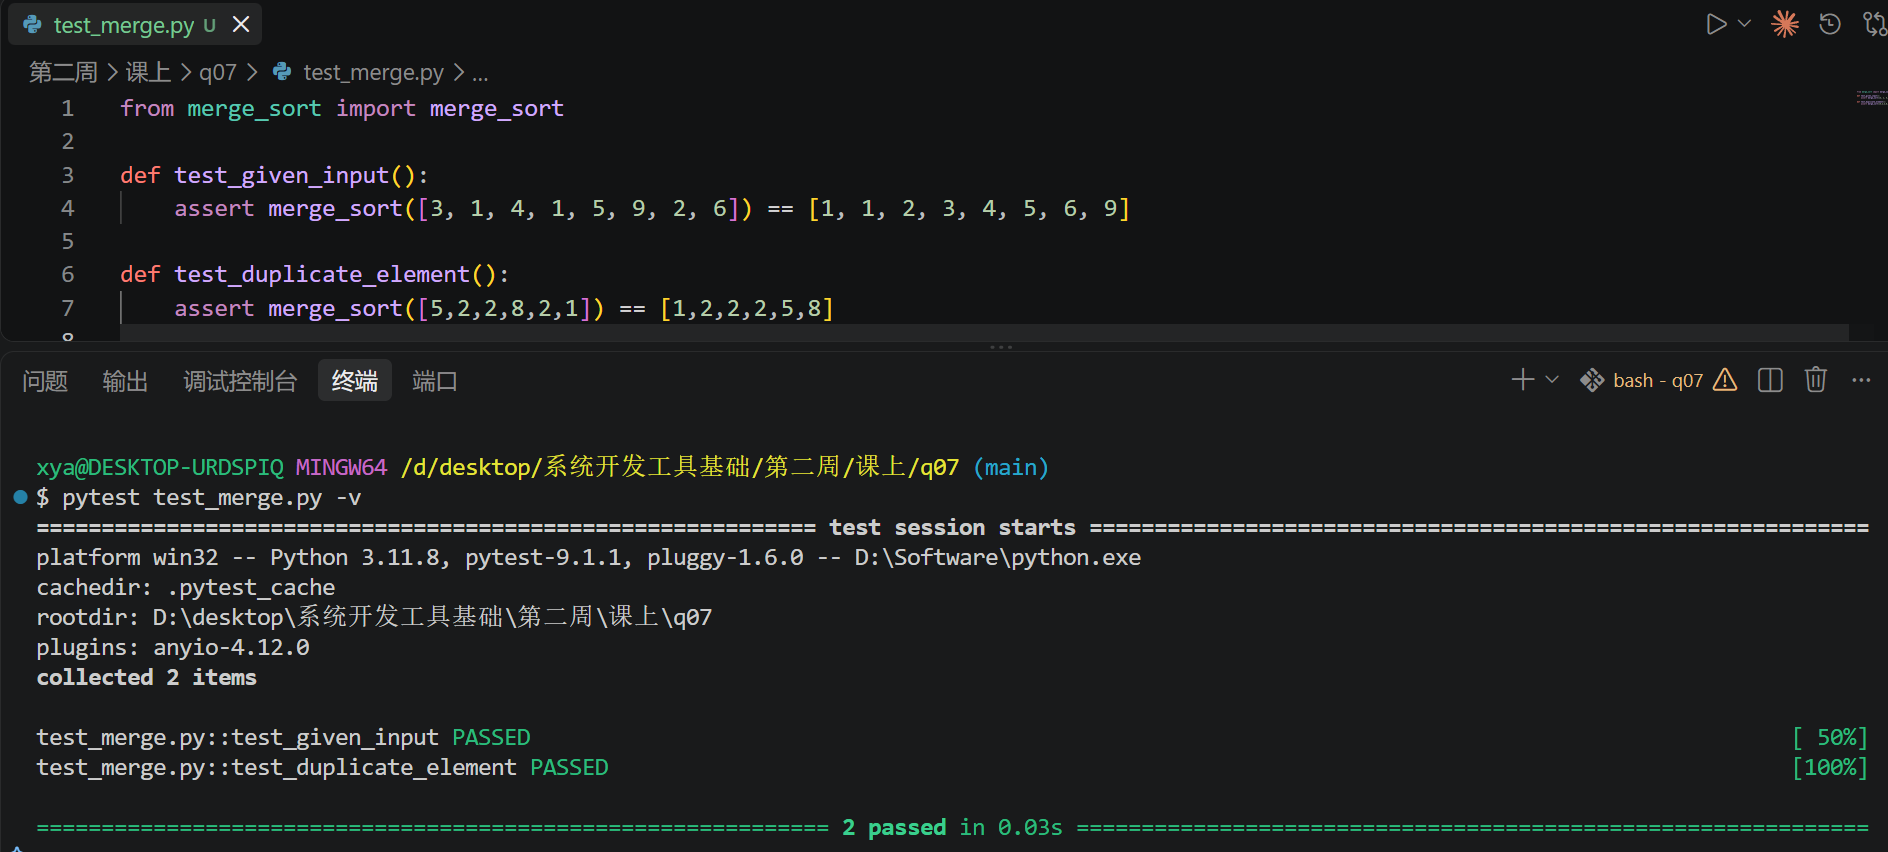
\includegraphics[width=0.96\textwidth]{课上/q07/图5-新增测试文件并且通过.png}
  \caption{两个归并排序测试均通过}
  \label{fig:q07-test}
\end{figure}

\textbf{实验结果：} pytest 共收集 2 个测试，给定输入和重复元素用例全部通过，
耗时 0.03 s（图~\ref{fig:q07-test}）。

\FloatBarrier

% ================= q08 =================
\subsection{q08 · 先测量，再优化慢速词频程序（Profiling）}

\begin{taskbox}[题目要求]
生成固定的 30000 个单词输入，测量并优化低效去重程序：
\begin{itemize}[nosep]
  \item 使用 \texttt{time} 运行原程序 2 次并记录耗时；
  \item 使用 \texttt{cProfile -s cumulative} 运行一次，找出主要耗时位置；
  \item 在不改变最终 count 的前提下优化程序，且不得写死 1000；
  \item 使用相同输入再运行 2 次，计算优化前后中位数和加速比。
\end{itemize}
\end{taskbox}

\textbf{实验过程：} 先运行 \texttt{generate\_words.py}，生成可重复使用的 \texttt{words.txt}。

\lstinputlisting[language=py,caption={generate\_words.py：生成固定随机词表},label={lst:q08-generate}]{课上/q08/generate_words.py}

使用 \texttt{time} 命令运行程序，两次 real 时间分别为 0.423 s 和 0.398 s，
输出计数均为 1000，见图~\ref{fig:q08-time}(a)。

\texttt{python -m cProfile -s cumulative wordfreq.py} 显示程序共运行 0.205 s，
其中顶层模块 \texttt{wordfreq.py:1(<module>)} 的累计时间为 0.203 s，文件读取和
\texttt{split} 只占 0.002 s（图~\ref{fig:q08-profile}）。耗时主要集中在模块内反复执行的
列表成员查找，而不是读取输入文件。

\begin{figure}[htbp]
  \centering
  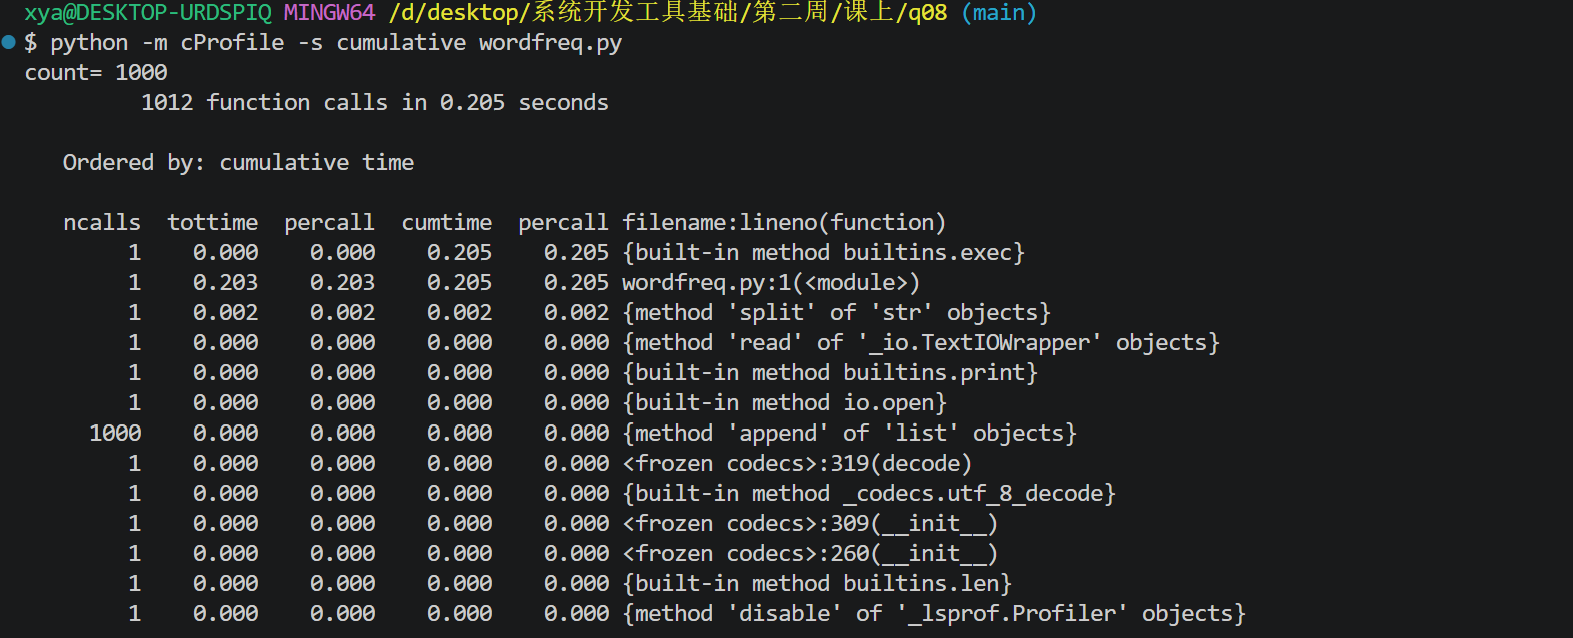
\includegraphics[width=0.96\textwidth]{课上/q08/图2-cProfile.png}
  \caption{cProfile 按累计时间排序的分析结果}
  \label{fig:q08-profile}
\end{figure}

将 \texttt{unique} 改成集合后，每个单词直接使用 \texttt{add} 加入集合，优化后的完整程序见代码~\ref{lst:q08-wordfreq}。

\lstinputlisting[language=py,caption={wordfreq.py：使用集合完成去重},label={lst:q08-wordfreq}]{课上/q08/wordfreq.py}

使用同一个 \texttt{words.txt} 再运行两次，real 时间分别为 0.207 s 和 0.221 s，
两次输出的计数仍为 1000，见图~\ref{fig:q08-time}(b)。

\begin{figure}[htbp]
  \centering
  \begin{minipage}[t]{0.49\textwidth}
    \centering
    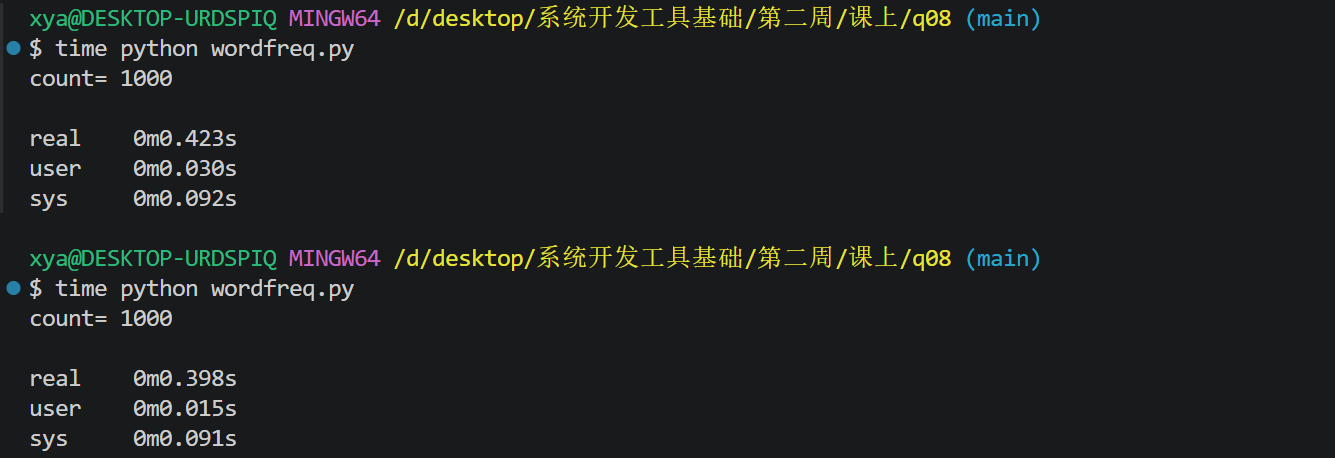
\includegraphics[width=\textwidth]{课上/q08/图1-原版时间.png}\\[-0.1em]
    \small (a) 原程序两次运行时间
  \end{minipage}\hfill
  \begin{minipage}[t]{0.49\textwidth}
    \centering
    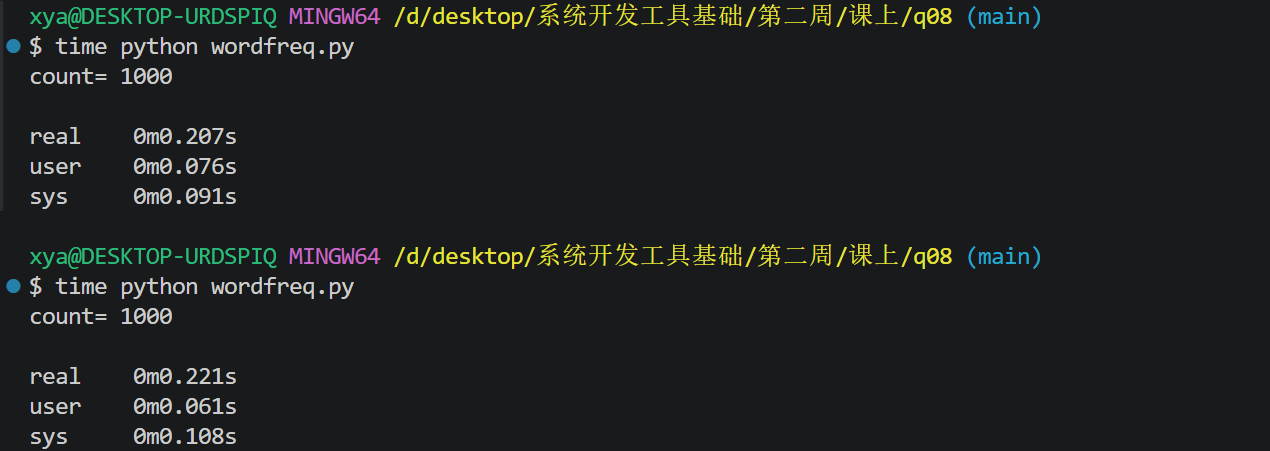
\includegraphics[width=\textwidth]{课上/q08/图3-改版时间.png}\\[-0.1em]
    \small (b) 集合优化后的两次运行时间
  \end{minipage}
  \caption{q08 使用相同输入优化前后的计时结果}
  \label{fig:q08-time}
\end{figure}

\begin{table}[htbp]
  \centering
  \caption{q08 优化前后运行时间与加速比}
  \label{tab:q08-time}
  \begin{tabular}{lccc}
    \toprule
    版本 & 第 1 次 / s & 第 2 次 / s & 中位数 / s \\
    \midrule
    列表去重 & 0.423 & 0.398 & 0.4105 \\
    集合去重 & 0.207 & 0.221 & 0.2140 \\
    \bottomrule
  \end{tabular}
\end{table}

\textbf{实验结果：} 两次测量的中位数分别为
\((0.423+0.398)/2=0.4105\) s 和 \((0.207+0.221)/2=0.2140\) s，
加速比为 \(0.4105/0.2140\approx1.92\)。优化后运行时间约为原来的 52\%，
同时计数仍为 1000。完整计时对比见表~\ref{tab:q08-time}。

\FloatBarrier

\section{课后练习}

\paragraph{参考资料记录}
\href{https://missing-semester-cn.github.io/2026/command-line-environment/}{Missing Semester：命令行环境}、
\href{https://missing-semester-cn.github.io/2026/development-environment/}{Missing Semester：开发环境与工具}、
\href{https://missing-semester-cn.github.io/2020/editors/}{Missing Semester：编辑器（Vim）}、
\href{https://missing-semester-cn.github.io/2026/debugging-profiling/}{Missing Semester：Debugging and Profiling}。

% 图片可以在当前板块内浮动，以填补页尾空白；每节末尾用 FloatBarrier 限制范围。
\setcounter{topnumber}{4}
\setcounter{bottomnumber}{3}
\setcounter{totalnumber}{6}
\renewcommand{\topfraction}{0.95}
\renewcommand{\bottomfraction}{0.85}
\renewcommand{\textfraction}{0.05}
\renewcommand{\floatpagefraction}{0.78}
\newcommand{\practiceimage}[4]{%
  \begin{figure}[!htbp]
    \centering
    \includegraphics[width=#1\textwidth]{\detokenize{#2}}
    \caption{#3}
    \label{#4}
  \end{figure}
}

\subsection{命令行环境}

\noindent\textbf{1．多参数与花括号展开。}
使用 \texttt{mkdir -p demo/\{src,docs,logs\}} 一次建立三个子目录，再用
\texttt{touch demo/src/\{main,utils,test\}.py} 创建三个源码文件；
\texttt{find} 输出的目录树说明两次展开都符合预期，见图~\ref{fig:after-cli-1}。
\practiceimage{0.82}{课后/command-line/1多参数和花括号展开.png}{花括号展开创建练习目录与文件}{fig:after-cli-1}

\noindent\textbf{2．通配符展开。}
将 \texttt{demo/src/*.py} 交给 Shell 展开，\texttt{printf} 依次输出
\texttt{main.py}、\texttt{test.py} 和 \texttt{utils.py}，结果见图~\ref{fig:after-cli-2}。
\practiceimage{0.78}{课后/command-line/2通配符展开.png}{通配符匹配三个 Python 文件}{fig:after-cli-2}

\noindent\textbf{3．分离标准输出与标准错误。}
用文件描述符 1、2 分开输出：普通消息写入 \texttt{stdout.log}，警告消息写入
\texttt{stderr.log}；随后读取文件确认两路输出没有混在一起，见图~\ref{fig:after-cli-3}。
\practiceimage{0.88}{课后/command-line/3分离 stdout 和 stderr.png}{标准输出与标准错误分别写入日志}{fig:after-cli-3}

\noindent\textbf{4．使用管道处理数据流。}
把消息依次送入 \texttt{sort}、\texttt{uniq -c} 和 \texttt{sort -rn}，
再由 \texttt{tee} 同时显示并保存统计结果，最终 \texttt{error} 出现 3 次，见图~\ref{fig:after-cli-4}。
\practiceimage{0.88}{课后/command-line/4使用管道处理数据流.png}{管道完成消息频次统计}{fig:after-cli-4}

\noindent\textbf{5．比较单引号与双引号。}
对变量 \texttt{tool} 分别使用双引号和单引号，前者输出变量值 \texttt{ruff}，
后者保留字面量 \texttt{\$tool}，差别见图~\ref{fig:after-cli-5}。
\practiceimage{0.80}{课后/command-line/5比较单引号和双引号.png}{单引号与双引号的变量展开差异}{fig:after-cli-5}

\noindent\textbf{6．命令替换。}
在 \texttt{\$(...)} 中组合 \texttt{find} 和 \texttt{wc -l}，将统计值保存到
\texttt{py\_count}；输出 \texttt{python files=3} 与实际文件数一致，见图~\ref{fig:after-cli-6}。
\practiceimage{0.78}{课后/command-line/6命令替换.png}{命令替换获取 Python 文件数量}{fig:after-cli-6}

\noindent\textbf{7．进程替换。}
两个 \texttt{<(printf ...)} 分别产生一份临时输入供 \texttt{diff} 比较，
输出指出第二行分别是 \texttt{utils.py} 和 \texttt{test.py}；此时 \texttt{diff}
返回非零值只是表示发现差异，比较过程本身没有失败，见图~\ref{fig:after-cli-7}。
\practiceimage{0.82}{课后/command-line/7进程替换.png}{进程替换生成两路 diff 输入}{fig:after-cli-7}

\noindent\textbf{8．临时变量与导出变量。}
\texttt{COURSE\_MODE} 只对紧随其后的命令生效，父 Shell 中仍为 \texttt{unset}；
经 \texttt{export} 设置的 \texttt{COURSE\_WEEK} 能被子 Shell 读取，并在
\texttt{unset} 后消失，完整结果见图~\ref{fig:after-cli-8}。
\practiceimage{0.82}{课后/command-line/8临时环境变量与导出变量.png}{环境变量的作用范围与继承}{fig:after-cli-8}

\noindent\textbf{9．返回码与短路执行。}
\texttt{grep} 找到 \texttt{error} 后执行 \texttt{\&\&} 右侧命令，找不到
\texttt{fatal} 时执行 \texttt{||} 右侧命令；随后用 \texttt{\$?} 取得
\texttt{false} 的返回码 1，见图~\ref{fig:after-cli-9}。
\practiceimage{0.82}{课后/command-line/9返回码与短路执行.png}{条件执行与返回码检查}{fig:after-cli-9}

\noindent\textbf{10．获取后台 PID 并发送信号。}
后台启动 \texttt{sleep} 后用 \texttt{\$!} 保存其 PID，再发送 SIGTERM 并
\texttt{wait}；返回码 143 等于 \(128+15\)，说明进程确实由 15 号信号终止，见图~\ref{fig:after-cli-10}。
\practiceimage{0.82}{课后/command-line/10使用 $! 获取后台进程 PID 并发送信号.png}{向后台进程发送 SIGTERM}{fig:after-cli-10}

\noindent\textbf{11．查看命令行程序的信息。}
依次使用 \texttt{--version}、\texttt{--help} 和 \texttt{type -a} 查看 Python
版本、常用选项及系统中全部同名可执行文件位置，结果见图~\ref{fig:after-cli-11}。
\practiceimage{0.88}{课后/command-line/11查看 CLI 常见选项和程序位置.png}{Python 的版本、帮助与程序位置}{fig:after-cli-11}

\FloatBarrier

\subsection{开发环境与工具}

前七项在 VS Code 中观察语言服务器和扩展提供的开发功能，后三项改用 Vim
完成同一个 FizzBuzz 文件的录入和修改，分别体验图形化 IDE 与终端编辑器的工作方式。

\noindent\textbf{1．查看 VS Code 与现有扩展。}
通过 \texttt{code --version} 查看编辑器版本，再筛选扩展列表，确认 Python、
debugpy 和 Pylance 已经安装，见图~\ref{fig:after-dev-1}。
\practiceimage{0.82}{课后/development/1查看 VS Code 和现有扩展.png}{VS Code 版本及 Python 开发扩展}{fig:after-dev-1}

\noindent\textbf{2．从命令行安装开发扩展。}
使用 \texttt{code --install-extension} 安装 Ruff 和 Error Lens，并再次查询扩展列表，
命令输出表明二者均安装成功。
\practiceimage{0.92}{课后/development/2从命令行安装开发扩展.png}{从命令行安装并确认开发扩展}{fig:after-dev-2}

\noindent\textbf{3．选择并验证 Python 解释器。}
在 VS Code 中按 \texttt{Ctrl+Shift+P} 打开命令面板，通过
\texttt{Python: Select Interpreter} 选择解释器，再在终端打印版本和路径；
最终使用 Python 3.11.8，位置为 \texttt{D:/Software/python.exe}，见图~\ref{fig:after-dev-3}。
\practiceimage{0.80}{课后/development/3选择并验证 Python 解释器（说明一下Ctrl+shift+P选择版本）.png}{终端验证 VS Code 选用的 Python 解释器}{fig:after-dev-3}

下面几个实例使用带类型注解的 \texttt{Product} 类和 \texttt{total} 函数，
基础代码见代码~\ref{lst:after-dev-product}。

\lstinputlisting[language=py,caption={Product 数据类与总价函数},label={lst:after-dev-product}]{课后/development/product.py}

\noindent\textbf{4．语义代码补全。}
在 \texttt{Product} 对象 \texttt{first} 后输入点号，Pylance 根据类定义给出
\texttt{name}、\texttt{price} 等成员候选，不需要手工记忆属性名，见图~\ref{fig:after-dev-4}。
\practiceimage{0.82}{课后/development/4演示语义代码补全.png}{Pylance 根据对象类型补全成员}{fig:after-dev-4}

\noindent\textbf{5．查看函数签名。}
将光标停在 \texttt{total(items)} 调用处，悬停信息显示参数为
\texttt{list[Product]}、返回值为 \texttt{float}，见图~\ref{fig:after-dev-5}。
\practiceimage{0.72}{课后/development/5查看函数签名.png}{查看 total 函数的类型签名}{fig:after-dev-5}

\noindent\textbf{6．调用 Quick Fix 修复缺失导入。}
直接使用 \texttt{datetime.now()} 时，Pylance 标出未定义名称；按提示调出
Quick Fix 后出现自动补充导入的修复入口，过程见图~\ref{fig:after-dev-6}。
\practiceimage{0.78}{课后/development/6使用 Quick Fix 自动补充缺失导入.png}{未定义名称对应的 Quick Fix 入口}{fig:after-dev-6}

\noindent\textbf{7．使用类型检查发现参数错误。}
把字符串 \texttt{"39.9"} 传给要求 \texttt{float} 的 \texttt{price} 参数，
Pylance 在运行前便报告 \texttt{reportArgumentType}，具体提示见图~\ref{fig:after-dev-7}。
\practiceimage{0.84}{课后/development/7使用类型检查发现参数类型错误.png}{Pylance 报告参数类型不兼容}{fig:after-dev-7}

\noindent\textbf{8．使用 Vim 创建并保存文件。}
在 Vim 中按 \texttt{i} 进入插入模式并录入 FizzBuzz 程序，按 Esc 回到正常模式，
再在命令行模式输入 \texttt{:w}。图~\ref{fig:after-dev-8} 记录了执行保存前的状态，
按下回车后文件写入完成。
\practiceimage{0.72}{课后/development/8使用Vim创建并保存Python文件.png}{在 Vim 中录入并保存 FizzBuzz 程序}{fig:after-dev-8}

\noindent\textbf{9．使用搜索和移动命令修改代码。}
先用 \texttt{/range} 搜索到循环范围，再用 \texttt{2w} 移到 \texttt{limit}，
配合 \texttt{i}、\texttt{e} 和 \texttt{a} 在两侧补入边界，最终得到
\texttt{range(1, limit + 1)}，见图~\ref{fig:after-dev-9}。
\practiceimage{0.72}{课后/development/9使用搜索和移动命令修改循环范围（过程记得写一下）.png}{使用 Vim 搜索与移动命令修改循环范围}{fig:after-dev-9}

\noindent\textbf{10．使用文本对象修改字符串。}
跳转到 5 的倍数所在分支后，用 \texttt{f"} 找到引号，再以 \texttt{ci"}
一次替换引号内部内容，将错误的 \texttt{fizz} 改为 \texttt{buzz}，见图~\ref{fig:after-dev-10}。
\practiceimage{0.68}{课后/development/10使用文本对象修改字符串（自己补过程）.png}{使用 Vim 文本对象替换字符串}{fig:after-dev-10}

\FloatBarrier

\subsection{Debugging and Profiling}

这一部分先围绕错误的平均值函数完成调试，再围绕队列实现完成性能分析。
前四项按“复现问题、观察异常、定位原因、修复验证”的顺序进行；确认程序正确后，
再从单次测量、重复基准测试、函数级分析和规模变化几个角度比较性能。

\subsubsection*{Debugging}

\noindent\textbf{1．复现错误并查看调试日志。}
原程序计算 \texttt{[10,20,30,40]} 的平均值时输出 33.33，而逐项写入的 DEBUG
日志表明累计和为 100，因此求和过程正常，问题更可能出在最后的除法，见图~\ref{fig:after-dp-1}。
\practiceimage{0.84}{课后/debugging_and_profiling/1复现结果并查看调试日志.png}{错误结果及逐项累加日志}{fig:after-dp-1}

\noindent\textbf{2．使用边界输入观察异常栈。}
把输入缩小为单元素列表 \texttt{[10]} 后，原返回语句把 \texttt{len(values)}
减 1 后作为分母，此时分母变为 0，程序触发除零异常；异常栈直接指向平均值函数
第 11 行，见图~\ref{fig:after-dp-2}。
\practiceimage{0.84}{课后/debugging_and_profiling/2制造边界输入并查看异常栈.png}{单元素输入触发的 ZeroDivisionError}{fig:after-dp-2}

\noindent\textbf{3．使用 pdb 检查变量并定位错误。}
在返回语句设置断点后，\texttt{pdb} 显示总和为 100、列表长度为 4；
正确结果应为 \(100/4=25\)，而原表达式实际使用分母 3；
这些运行时数据确认错误来自多减的 1，见图~\ref{fig:after-dp-3}。
\practiceimage{0.78}{课后/debugging_and_profiling/3使用pdb检查变量并定位错误.png}{pdb 断点处的变量检查结果}{fig:after-dp-3}

\noindent\textbf{4．修复平均值错误并验证结果。}
将返回语句改为 \texttt{total/len(values)} 后重新测试，四个数的平均值变为 25.00，
单元素列表也能正确返回 10.0，完成了从复现、定位到修复的闭环，见图~\ref{fig:after-dp-4}；
修复后的程序见代码~\ref{lst:after-dp-stats}。
\practiceimage{0.76}{课后/debugging_and_profiling/4修复平均值错误并验证结果.png.png}{修复后普通输入与边界输入均得到正确结果}{fig:after-dp-4}

\lstinputlisting[language=py,caption={修复后的平均值程序},label={lst:after-dp-stats}]{课后/debugging_and_profiling/stats_bug.py}

\subsubsection*{Profiling}

后续实例比较两种队列：\texttt{list\_queue} 每次删除列表首元素，
\texttt{deque\_queue} 则调用双端队列的 \texttt{popleft}。用于计时与内存测量的完整程序见
代码~\ref{lst:after-dp-queue}。

\lstinputlisting[language=py,caption={list 与 deque 队列性能测试程序},label={lst:after-dp-queue}]{课后/debugging_and_profiling/queue_bench.py}

\noindent\textbf{5．比较运行时间与峰值内存。}
两种实现处理 50000 个元素后都得到 \texttt{1249975000}，说明功能一致；
本次测量中 list 用时 0.327324 s，deque 用时 0.085437 s，峰值内存都约为 1.9 MiB，见图~\ref{fig:after-dp-5}。
\practiceimage{0.84}{课后/debugging_and_profiling/5比较list和deque的时间与内存.png}{两种队列的单次时间与峰值内存}{fig:after-dp-5}

\noindent\textbf{6．使用 timeit 重复测量。}
为减小单次计时的偶然误差，分别进行 5 轮、每轮 3 次测量；list 每次约 233 ms，
deque 每次约 4.28 ms，前者约为后者的 54 倍，见图~\ref{fig:after-dp-6}。
\practiceimage{0.82}{课后/debugging_and_profiling/6使用timeit重复测量两种队列.png}{timeit 重复测量 list 与 deque}{fig:after-dp-6}

\noindent\textbf{7．使用 cProfile 分析 list 热点。}
将分析数据保存为 \texttt{list.prof} 后用 \texttt{pstats} 按内部耗时排序；
50000 次 \texttt{list.pop} 共占 0.233 s，是 list 版本最明显的热点，见图~\ref{fig:after-dp-7}。
\practiceimage{0.82}{课后/debugging_and_profiling/7使用cProfile分析list热点.png}{list 版本的 cProfile 统计}{fig:after-dp-7}

\noindent\textbf{8．使用 cProfile 分析 deque 热点。}
以相同参数分析 deque 版本时，50000 次 \texttt{popleft} 只占 0.006 s，
整个分析过程也由 list 的 0.351 s 降至 0.117 s，两份报告的差异见图~\ref{fig:after-dp-8}。
\practiceimage{0.82}{课后/debugging_and_profiling/8使用cProfile分析deque热点.png}{deque 版本的 cProfile 统计}{fig:after-dp-8}

\noindent\textbf{9．测量不同数据规模下的性能。}
为了观察增长趋势，使用代码~\ref{lst:after-dp-scaling} 对 5000、10000、20000、40000
四种规模各重复测量 5 次并取中位数，再把结果写入 CSV；数据规模每翻倍，list 用时接近
增长 4 倍，而 deque 的增长更接近线性，见图~\ref{fig:after-dp-9}。

\lstinputlisting[language=py,caption={多种数据规模的重复计时程序},label={lst:after-dp-scaling}]{课后/debugging_and_profiling/scaling.py}

\practiceimage{0.78}{课后/debugging_and_profiling/9测量不同规模下的队列性能.png}{不同队列规模对应的计时数据}{fig:after-dp-9}

\noindent\textbf{10．绘制性能变化曲线。}
读取上一步生成的 \texttt{queue\_scaling.csv}，用 Matplotlib 将两组中位数绘制为折线；
list 曲线随规模快速上升，而 deque 始终贴近横轴，图形与前面的计时和热点分析一致，见图~\ref{fig:after-dp-10}。
\practiceimage{0.72}{课后/debugging_and_profiling/10queue_scaling.png}{list.pop(0) 与 deque.popleft() 的性能曲线}{fig:after-dp-10}

\noindent\textbf{11．查找占用端口的进程并释放端口。}
启动 4444 端口上的临时 HTTP 服务后，\texttt{netstat -ano} 找到监听进程 PID 55428；
停止服务并再次查询时已无监听记录，终端输出 \texttt{port 4444 released}，见图~\ref{fig:after-dp-11}。
\practiceimage{0.88}{课后/debugging_and_profiling/11查找端口占用进程并释放端口.png}{定位端口监听进程并确认端口释放}{fig:after-dp-11}

\FloatBarrier

\section{解题感悟}

先记录一下这周学会了什么吧。命令行环境这部分以前接触得比较零散，之前大概会些常用的文本操作和一些简单的脚本命令吧，
这次好好巩固了第一周的shell和各种脚本语言，延申了进程、ssh等知识点，明显感觉到shell比之前想的要厉害得多，
比如说控制命令之间怎么传数据、程序在什么环境里运行，以及后台任务什么时候结束等。
有些符号现在还是容易混，之后真用到估计还是得再查一下。

开发环境这部分让我重新认识了一下平时一直在用的 VS Code。之前的话写代码其实写的都比较简单没好好了解 IDE 的功能，
更多是把补全和报错提示当成编辑器自带的功能，这次才知道解释器、Python 扩展和 Pylance 各自在做什么。
中间还装了 Ruff 和 Error Lens 试了一下，Error Lens 把提示直接铺在代码后面看得太烦了，所以实验完成后还是卸载了。
Vim 刚开始用挺不习惯的，有命令要记得都挺烦的，熟练以后应该会比一直移动光标快很多。

这周的 Debugging 和 Profiling 部分让我更熟悉了调试方式吧，对性能的分析也更加重视了。
之前打断点调试不是很熟练，这次练习了两种调试方式；
性能分析也让我发现“感觉哪个写法快”其实不太可靠，list 和 deque 在数据量小时看起来区别不大，
但用 timeit 重复测量、再看 cProfile 的热点和不同规模下的曲线，差距就很明显了。
以后再碰到程序慢的问题，应该先测一下到底慢在哪里，而不是上来就凭感觉改一堆代码。

现在遇到报错我还是习惯性想问 ai，不过之后至少应该先自己看看异常栈、变量值和性能数据，知道问题大概出在哪，
再让 ai 帮我解释或者找其它可能。

第二周课上实验、课后练习及实验报告均已提交至 Git 仓库，相关提交记录见图~\ref{fig:commit-record}。

\begin{center}
  
\includegraphics[width=\textwidth]{commit记录.png}
  \captionof{figure}{第二周实验及报告的 Git 提交记录}
  \label{fig:commit-record}
\end{center}

\end{document}
